% Options for packages loaded elsewhere
\PassOptionsToPackage{unicode}{hyperref}
\PassOptionsToPackage{hyphens}{url}
\PassOptionsToPackage{dvipsnames,svgnames,x11names}{xcolor}
%
\documentclass[
]{article}

\usepackage{amsmath,amssymb}
\usepackage{iftex}
\ifPDFTeX
  \usepackage[T1]{fontenc}
  \usepackage[utf8]{inputenc}
  \usepackage{textcomp} % provide euro and other symbols
\else % if luatex or xetex
  \usepackage{unicode-math}
  \defaultfontfeatures{Scale=MatchLowercase}
  \defaultfontfeatures[\rmfamily]{Ligatures=TeX,Scale=1}
\fi
\usepackage{lmodern}
\ifPDFTeX\else  
    % xetex/luatex font selection
\fi
% Use upquote if available, for straight quotes in verbatim environments
\IfFileExists{upquote.sty}{\usepackage{upquote}}{}
\IfFileExists{microtype.sty}{% use microtype if available
  \usepackage[]{microtype}
  \UseMicrotypeSet[protrusion]{basicmath} % disable protrusion for tt fonts
}{}
\makeatletter
\@ifundefined{KOMAClassName}{% if non-KOMA class
  \IfFileExists{parskip.sty}{%
    \usepackage{parskip}
  }{% else
    \setlength{\parindent}{0pt}
    \setlength{\parskip}{6pt plus 2pt minus 1pt}}
}{% if KOMA class
  \KOMAoptions{parskip=half}}
\makeatother
\usepackage{xcolor}
\setlength{\emergencystretch}{3em} % prevent overfull lines
\setcounter{secnumdepth}{5}
% Make \paragraph and \subparagraph free-standing
\makeatletter
\ifx\paragraph\undefined\else
  \let\oldparagraph\paragraph
  \renewcommand{\paragraph}{
    \@ifstar
      \xxxParagraphStar
      \xxxParagraphNoStar
  }
  \newcommand{\xxxParagraphStar}[1]{\oldparagraph*{#1}\mbox{}}
  \newcommand{\xxxParagraphNoStar}[1]{\oldparagraph{#1}\mbox{}}
\fi
\ifx\subparagraph\undefined\else
  \let\oldsubparagraph\subparagraph
  \renewcommand{\subparagraph}{
    \@ifstar
      \xxxSubParagraphStar
      \xxxSubParagraphNoStar
  }
  \newcommand{\xxxSubParagraphStar}[1]{\oldsubparagraph*{#1}\mbox{}}
  \newcommand{\xxxSubParagraphNoStar}[1]{\oldsubparagraph{#1}\mbox{}}
\fi
\makeatother


\providecommand{\tightlist}{%
  \setlength{\itemsep}{0pt}\setlength{\parskip}{0pt}}\usepackage{longtable,booktabs,array}
\usepackage{calc} % for calculating minipage widths
% Correct order of tables after \paragraph or \subparagraph
\usepackage{etoolbox}
\makeatletter
\patchcmd\longtable{\par}{\if@noskipsec\mbox{}\fi\par}{}{}
\makeatother
% Allow footnotes in longtable head/foot
\IfFileExists{footnotehyper.sty}{\usepackage{footnotehyper}}{\usepackage{footnote}}
\makesavenoteenv{longtable}
\usepackage{graphicx}
\makeatletter
\def\maxwidth{\ifdim\Gin@nat@width>\linewidth\linewidth\else\Gin@nat@width\fi}
\def\maxheight{\ifdim\Gin@nat@height>\textheight\textheight\else\Gin@nat@height\fi}
\makeatother
% Scale images if necessary, so that they will not overflow the page
% margins by default, and it is still possible to overwrite the defaults
% using explicit options in \includegraphics[width, height, ...]{}
\setkeys{Gin}{width=\maxwidth,height=\maxheight,keepaspectratio}
% Set default figure placement to htbp
\makeatletter
\def\fps@figure{htbp}
\makeatother

\usepackage{booktabs}
\usepackage{longtable}
\usepackage{array}
\usepackage{multirow}
\usepackage{wrapfig}
\usepackage{float}
\usepackage{colortbl}
\usepackage{pdflscape}
\usepackage{tabu}
\usepackage{threeparttable}
\usepackage{threeparttablex}
\usepackage[normalem]{ulem}
\usepackage{makecell}
\usepackage{xcolor}
\usepackage{booktabs}
\usepackage{longtable}
\usepackage[a4paper, left=0.75in, right=1in, top=1in, bottom=1in]{geometry}
\makeatletter
\@ifpackageloaded{caption}{}{\usepackage{caption}}
\AtBeginDocument{%
\ifdefined\contentsname
  \renewcommand*\contentsname{Table of contents}
\else
  \newcommand\contentsname{Table of contents}
\fi
\ifdefined\listfigurename
  \renewcommand*\listfigurename{List of Figures}
\else
  \newcommand\listfigurename{List of Figures}
\fi
\ifdefined\listtablename
  \renewcommand*\listtablename{List of Tables}
\else
  \newcommand\listtablename{List of Tables}
\fi
\ifdefined\figurename
  \renewcommand*\figurename{Figure}
\else
  \newcommand\figurename{Figure}
\fi
\ifdefined\tablename
  \renewcommand*\tablename{Table}
\else
  \newcommand\tablename{Table}
\fi
}
\@ifpackageloaded{float}{}{\usepackage{float}}
\floatstyle{ruled}
\@ifundefined{c@chapter}{\newfloat{codelisting}{h}{lop}}{\newfloat{codelisting}{h}{lop}[chapter]}
\floatname{codelisting}{Listing}
\newcommand*\listoflistings{\listof{codelisting}{List of Listings}}
\makeatother
\makeatletter
\makeatother
\makeatletter
\@ifpackageloaded{caption}{}{\usepackage{caption}}
\@ifpackageloaded{subcaption}{}{\usepackage{subcaption}}
\makeatother

\ifLuaTeX
  \usepackage{selnolig}  % disable illegal ligatures
\fi
\usepackage{bookmark}

\IfFileExists{xurl.sty}{\usepackage{xurl}}{} % add URL line breaks if available
\urlstyle{same} % disable monospaced font for URLs
\hypersetup{
  pdftitle={DAA path abundance},
  colorlinks=true,
  linkcolor={blue},
  filecolor={Maroon},
  citecolor={Blue},
  urlcolor={Blue},
  pdfcreator={LaTeX via pandoc}}


\title{DAA path abundance}
\author{}
\date{}

\begin{document}
\maketitle


\subsection{Differential abundance
analysis}\label{differential-abundance-analysis}

\begin{itemize}
\tightlist
\item
  Group variable: \textbf{diet}
\item
  Formula used: \textbf{\textasciitilde{} diet * timepoint + (1
  \textbar{} id)}
\end{itemize}

\begin{longtable}[t]{lrrrrrr}
\caption{Table of significant features}\\
\toprule
\textbf{feature} & \textbf{metadata} & \textbf{value} & \textbf{coef} & \textbf{qval\_individual} & \textbf{qval\_joint} & \textbf{model}\\
\midrule
\endfirsthead
\caption[]{Table of significant features \textit{(continued)}}\\
\toprule
\textbf{feature} & \textbf{metadata} & \textbf{value} & \textbf{coef} & \textbf{qval\_individual} & \textbf{qval\_joint} & \textbf{model}\\
\midrule
\endhead

\endfoot
\bottomrule
\endlastfoot
GALACTAR... & timepoint & after & 16.099 & 0.000 & 0.000 & prevalence\\
GLUCARGA... & timepoint & after & 16.099 & 0.000 & 0.000 & prevalence\\
GALACTAR... & diet & oat:timepointafter & -17.240 & 0.000 & 0.000 & prevalence\\
GLUCARGA... & diet & oat:timepointafter & -17.240 & 0.000 & 0.000 & prevalence\\
GLYCOLYS... & timepoint & after & -6.976 & 0.000 & 0.000 & prevalence\\
\addlinespace
FASYN.IN... & timepoint & after & -1.027 & 0.007 & 0.009 & abundance\\
PWY.622.... & timepoint & after & -0.837 & 0.034 & 0.023 & abundance\\
DAPLYSIN... & timepoint & after & -0.432 & 0.062 & 0.042 & abundance\\
PWY.7115... & timepoint & after & -0.733 & 0.080 & 0.055 & abundance\\
PWY0.106... & timepoint & after & -0.955 & 0.109 & 0.075 & abundance\\
\addlinespace
GALACTAR... & timepoint & after & -0.447 & 0.879 & 0.000 & abundance\\
GLUCARGA... & timepoint & after & -0.447 & 0.879 & 0.000 & abundance\\
GLYCOLYS... & timepoint & after & 2.528 & 0.898 & 0.000 & abundance\\
FASYN.IN... & timepoint & after & -3.102 & 0.907 & 0.009 & prevalence\\
GALACTAR... & diet & oat:timepointafter & 0.073 & 1.000 & 0.000 & abundance\\
\addlinespace
GLUCARGA... & diet & oat:timepointafter & 0.073 & 1.000 & 0.000 & abundance\\
PWY.622.... & timepoint & after & 0.000 & 1.000 & 0.023 & prevalence\\
DAPLYSIN... & timepoint & after & NA & NA & 0.042 & prevalence\\
PWY.7115... & timepoint & after & NA & NA & 0.055 & prevalence\\
PWY0.106... & timepoint & after & NA & NA & 0.075 & prevalence\\*
\end{longtable}

\begin{figure}[H]

{\centering 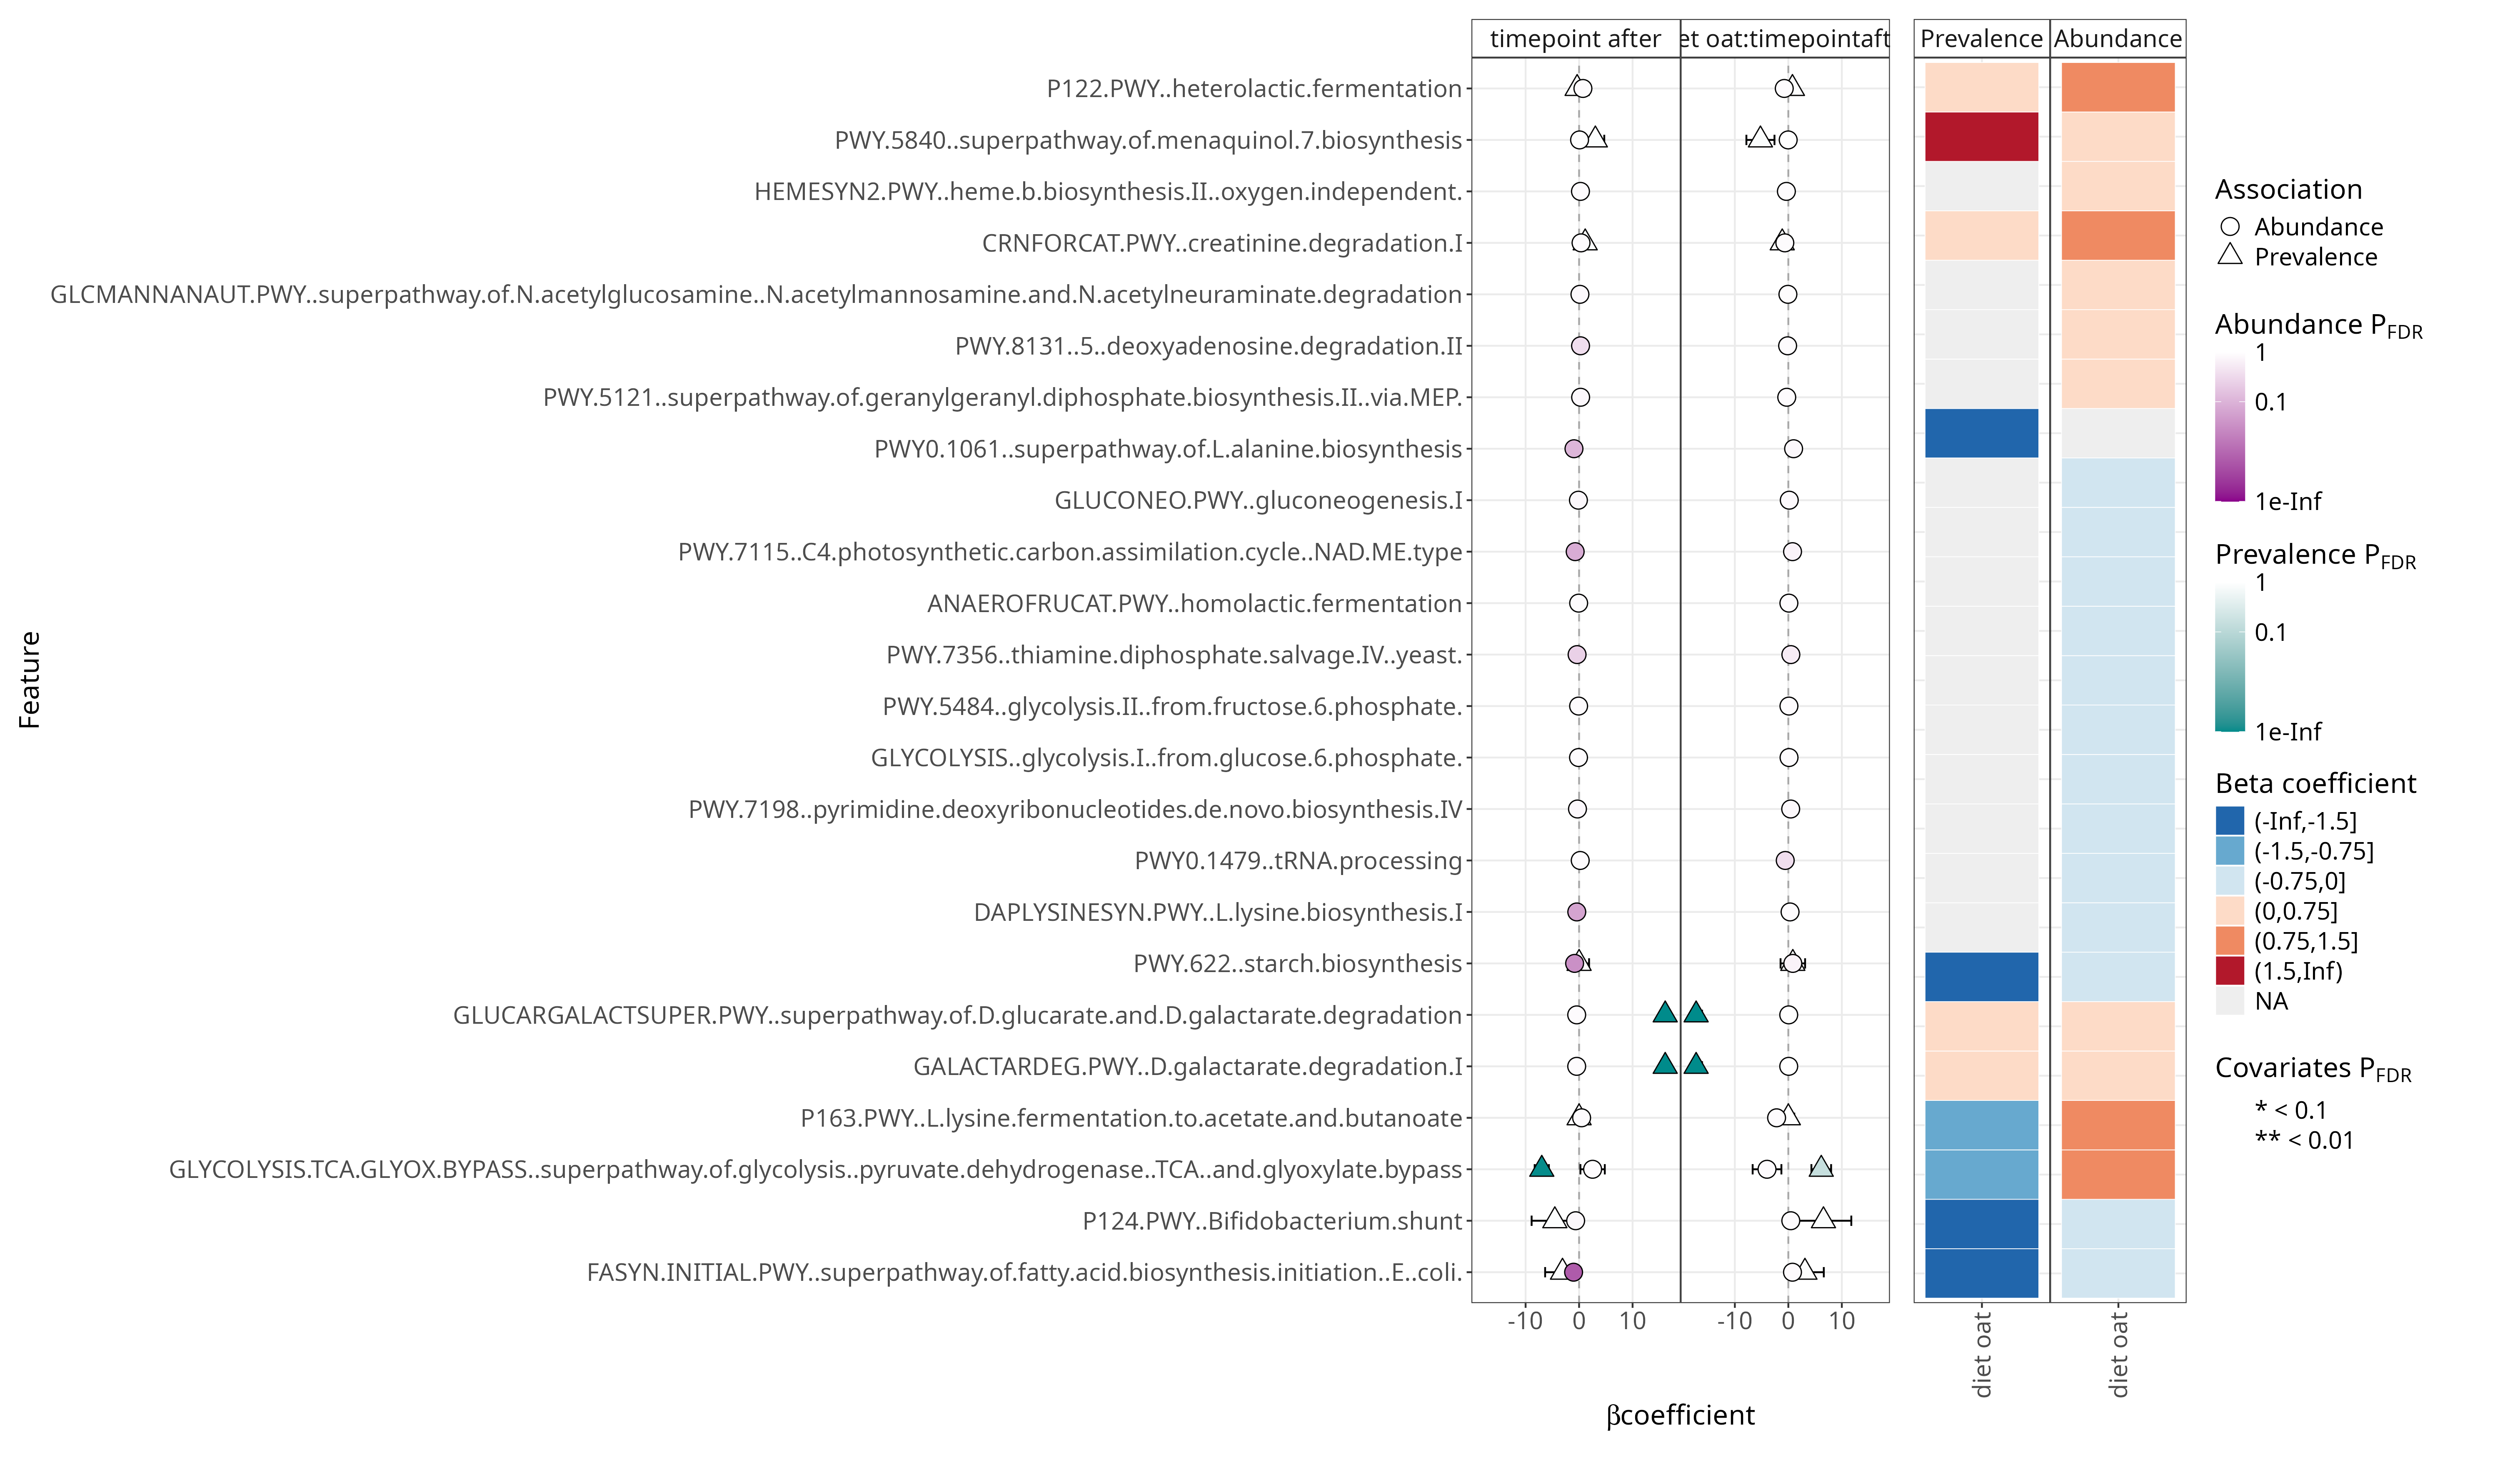
\includegraphics{../../output/daa/daa_pa/figures/summary_plot.png}

}

\caption{summary\_plot.png}

\end{figure}%

\begin{longtable}[]{@{}
  >{\raggedright\arraybackslash}p{(\columnwidth - 6\tabcolsep) * \real{0.2851}}
  >{\raggedright\arraybackslash}p{(\columnwidth - 6\tabcolsep) * \real{0.2337}}
  >{\raggedright\arraybackslash}p{(\columnwidth - 6\tabcolsep) * \real{0.2337}}
  >{\raggedright\arraybackslash}p{(\columnwidth - 6\tabcolsep) * \real{0.2476}}@{}}
\toprule\noalign{}
\endhead
\bottomrule\noalign{}
\endlastfoot
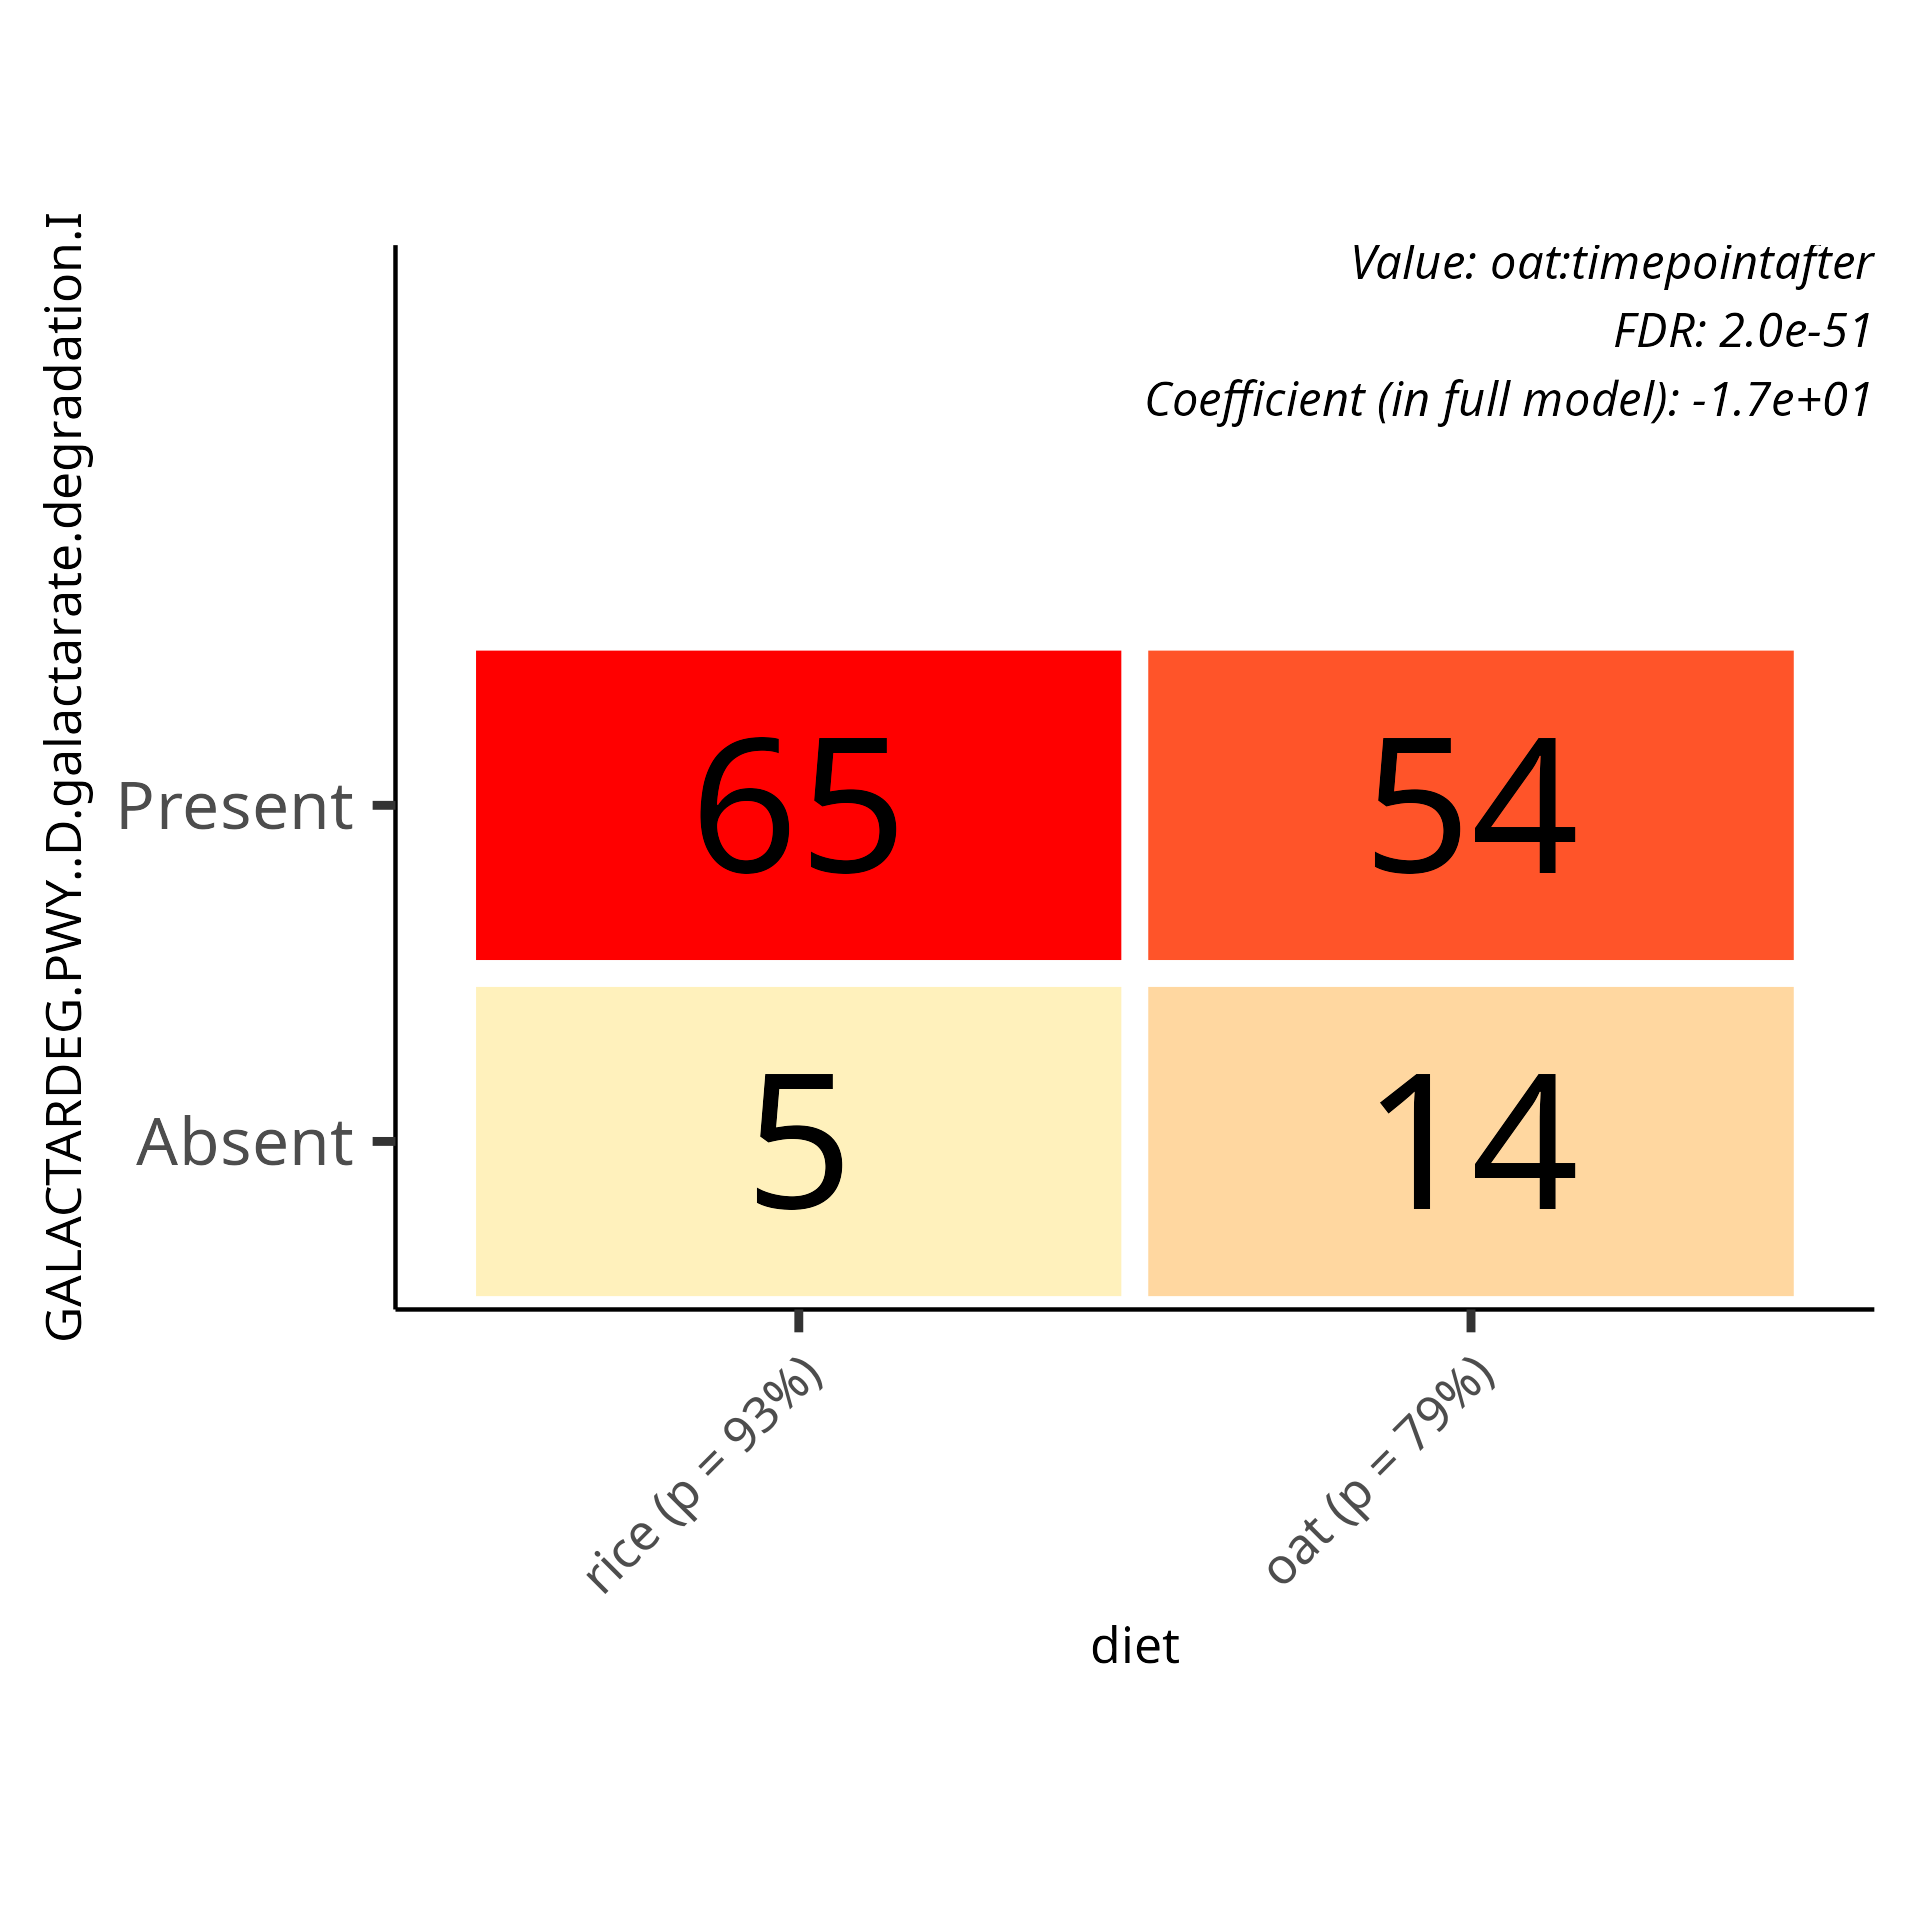
\includegraphics{../../output/daa/daa_pa/figures/association_plots/diet/logistic/diet_GALACTARDEG.PWY..D.galactarate.degradation.I_logistic.png}
&
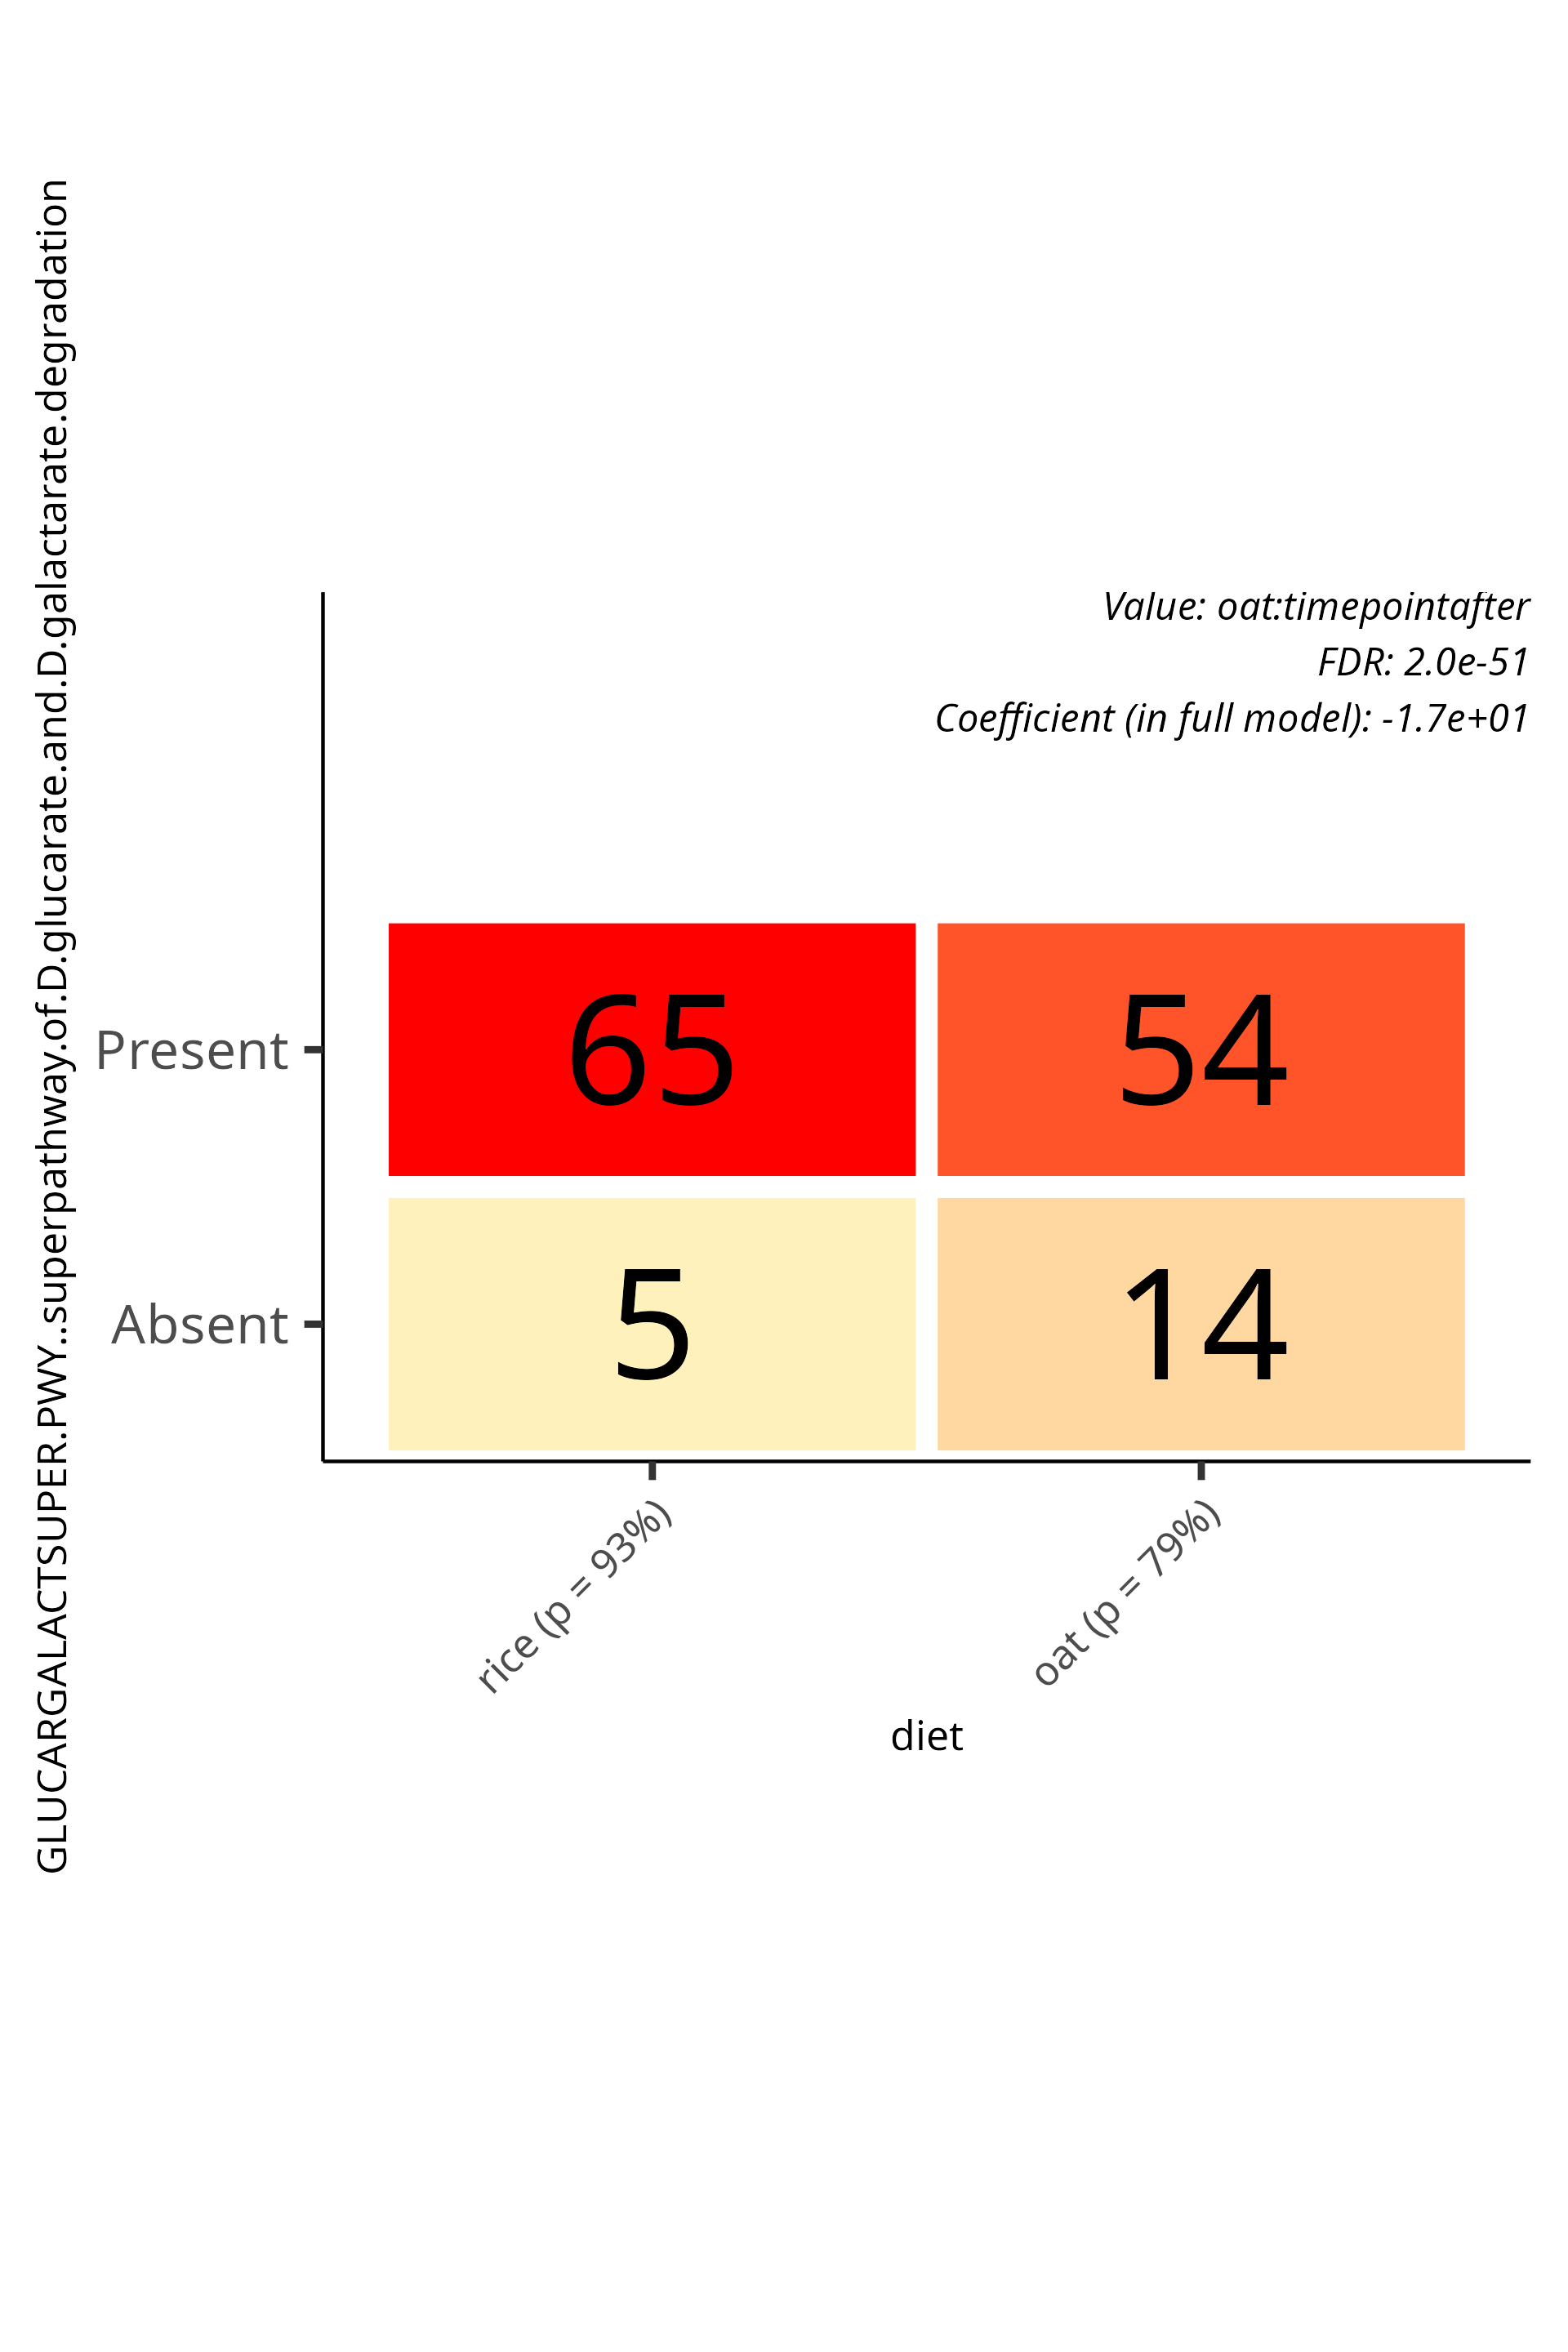
\includegraphics{../../output/daa/daa_pa/figures/association_plots/diet/logistic/diet_GLUCARGALACTSUPER.PWY..superpathway.of.D.glucarate.and.D.galactarate.degradation_logistic.png}
&
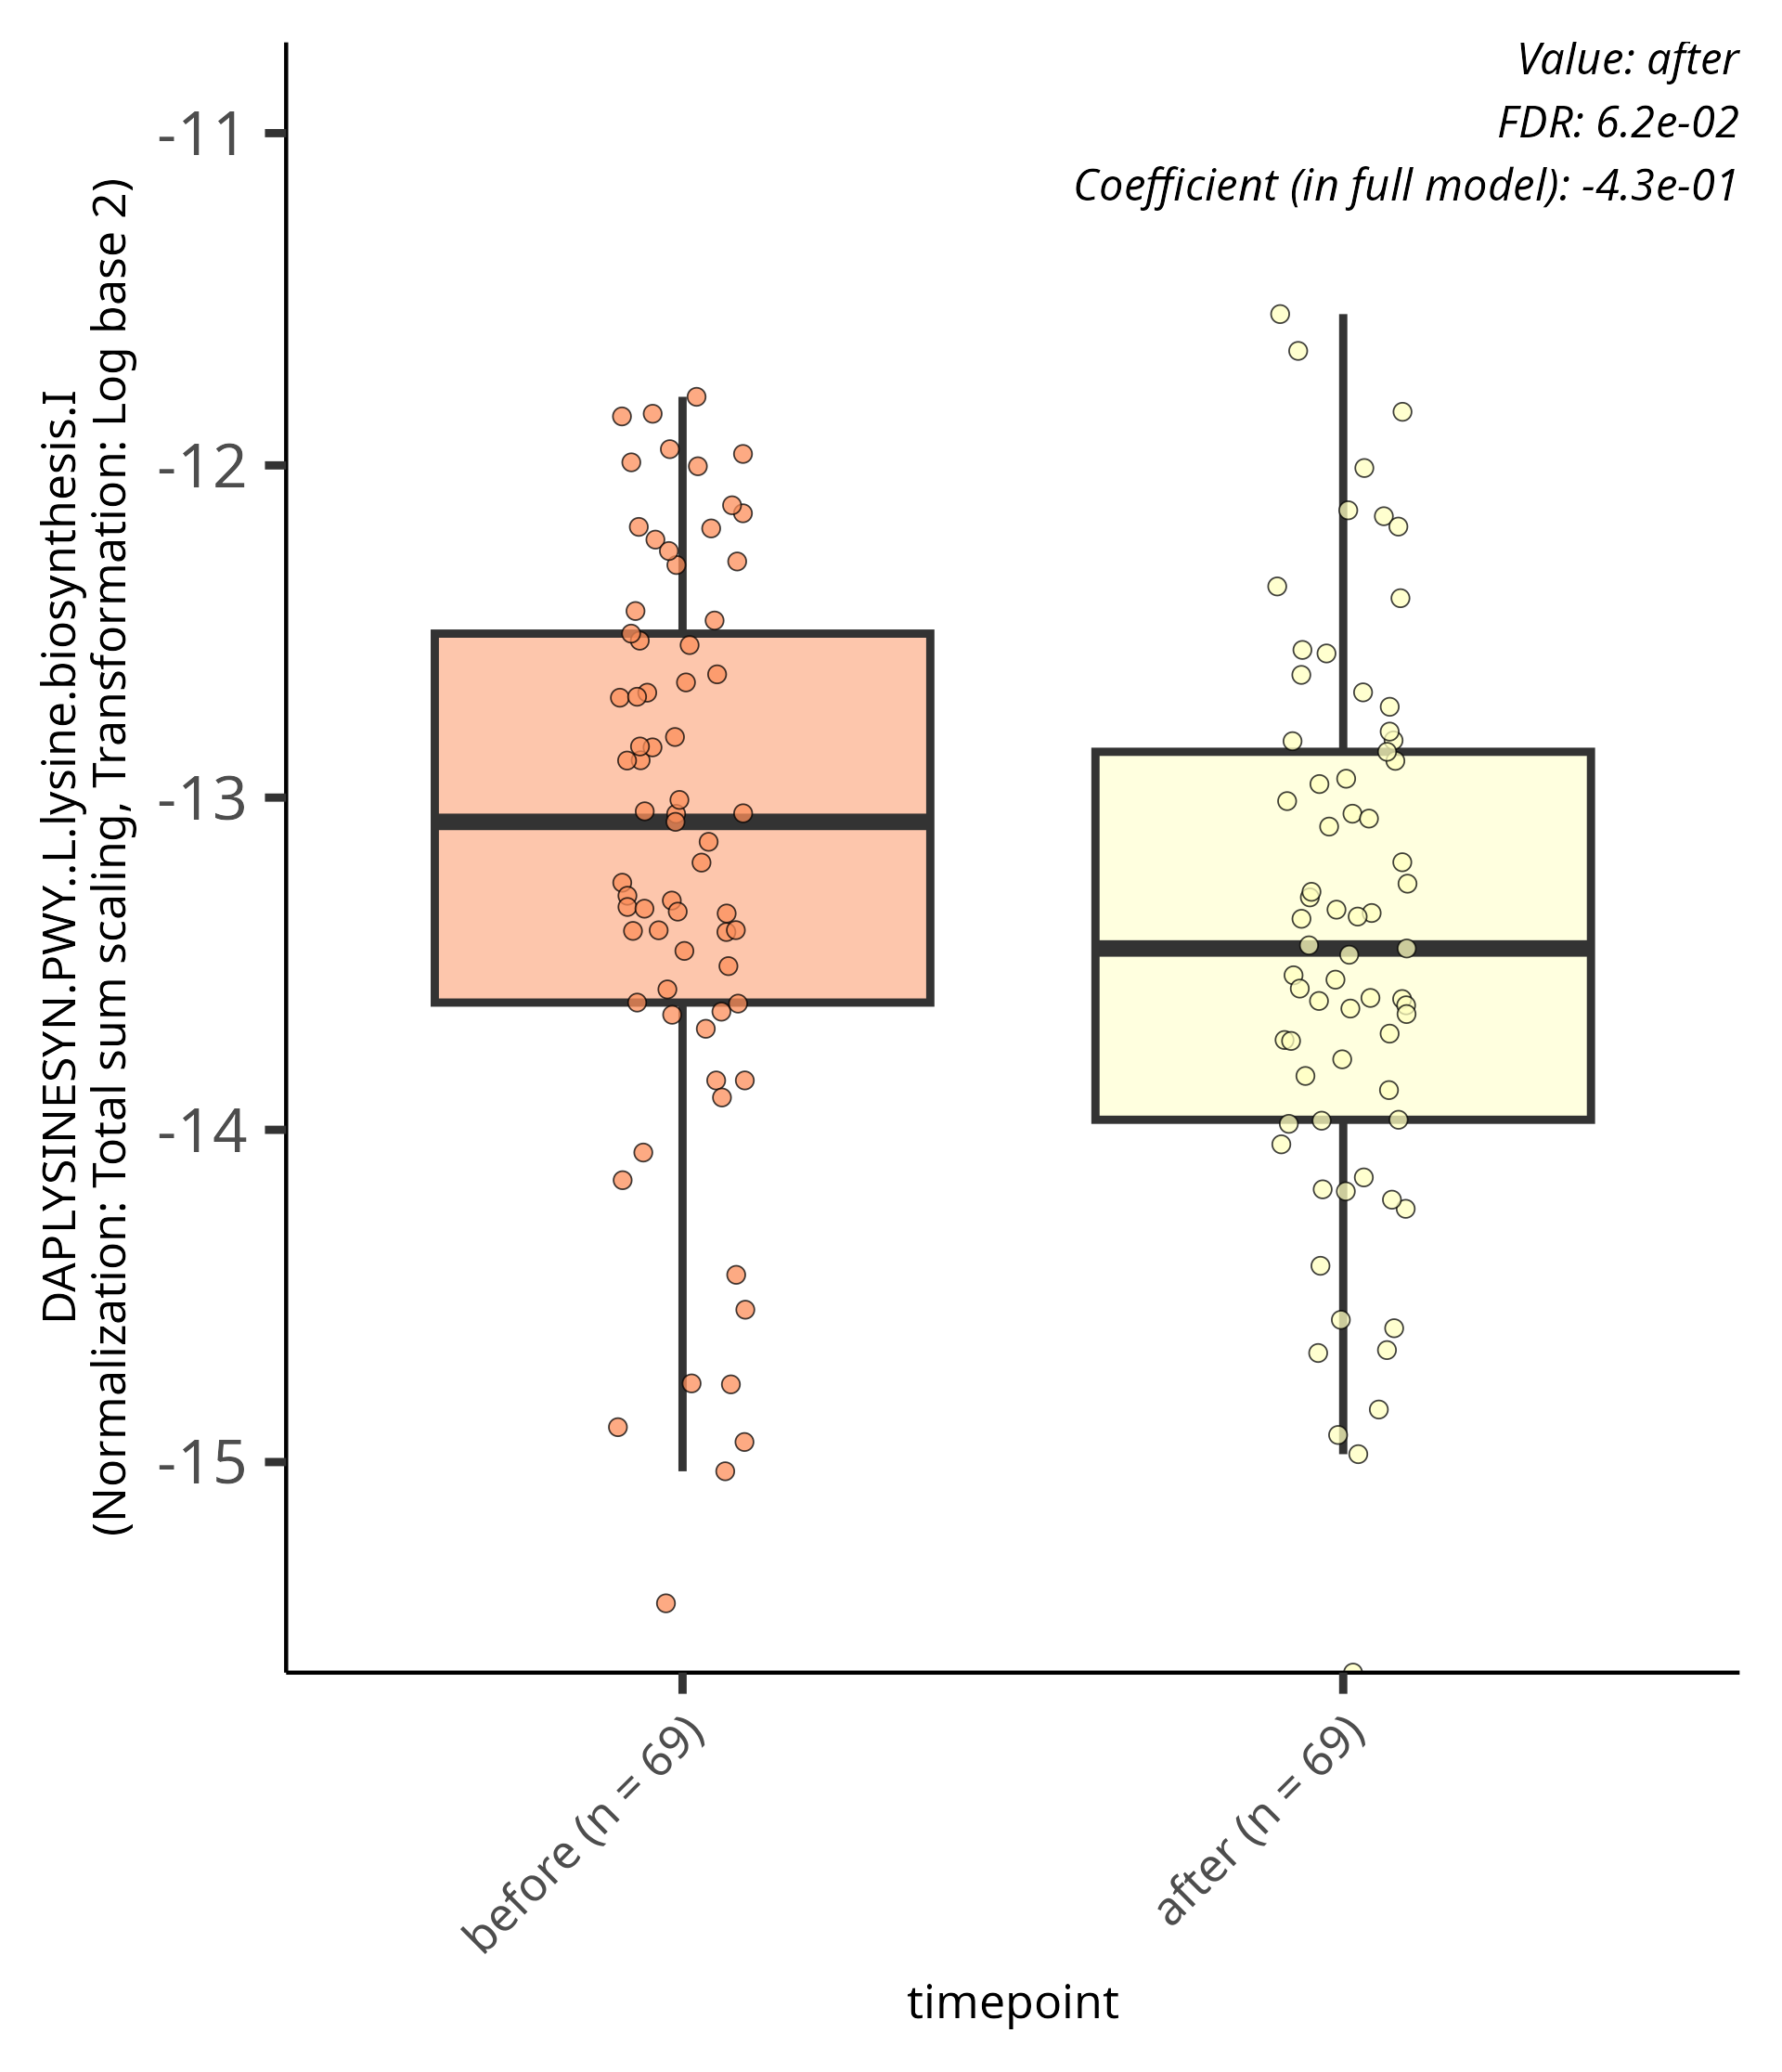
\includegraphics{../../output/daa/daa_pa/figures/association_plots/timepoint/linear/timepoint_DAPLYSINESYN.PWY..L.lysine.biosynthesis.I_linear.png}
&
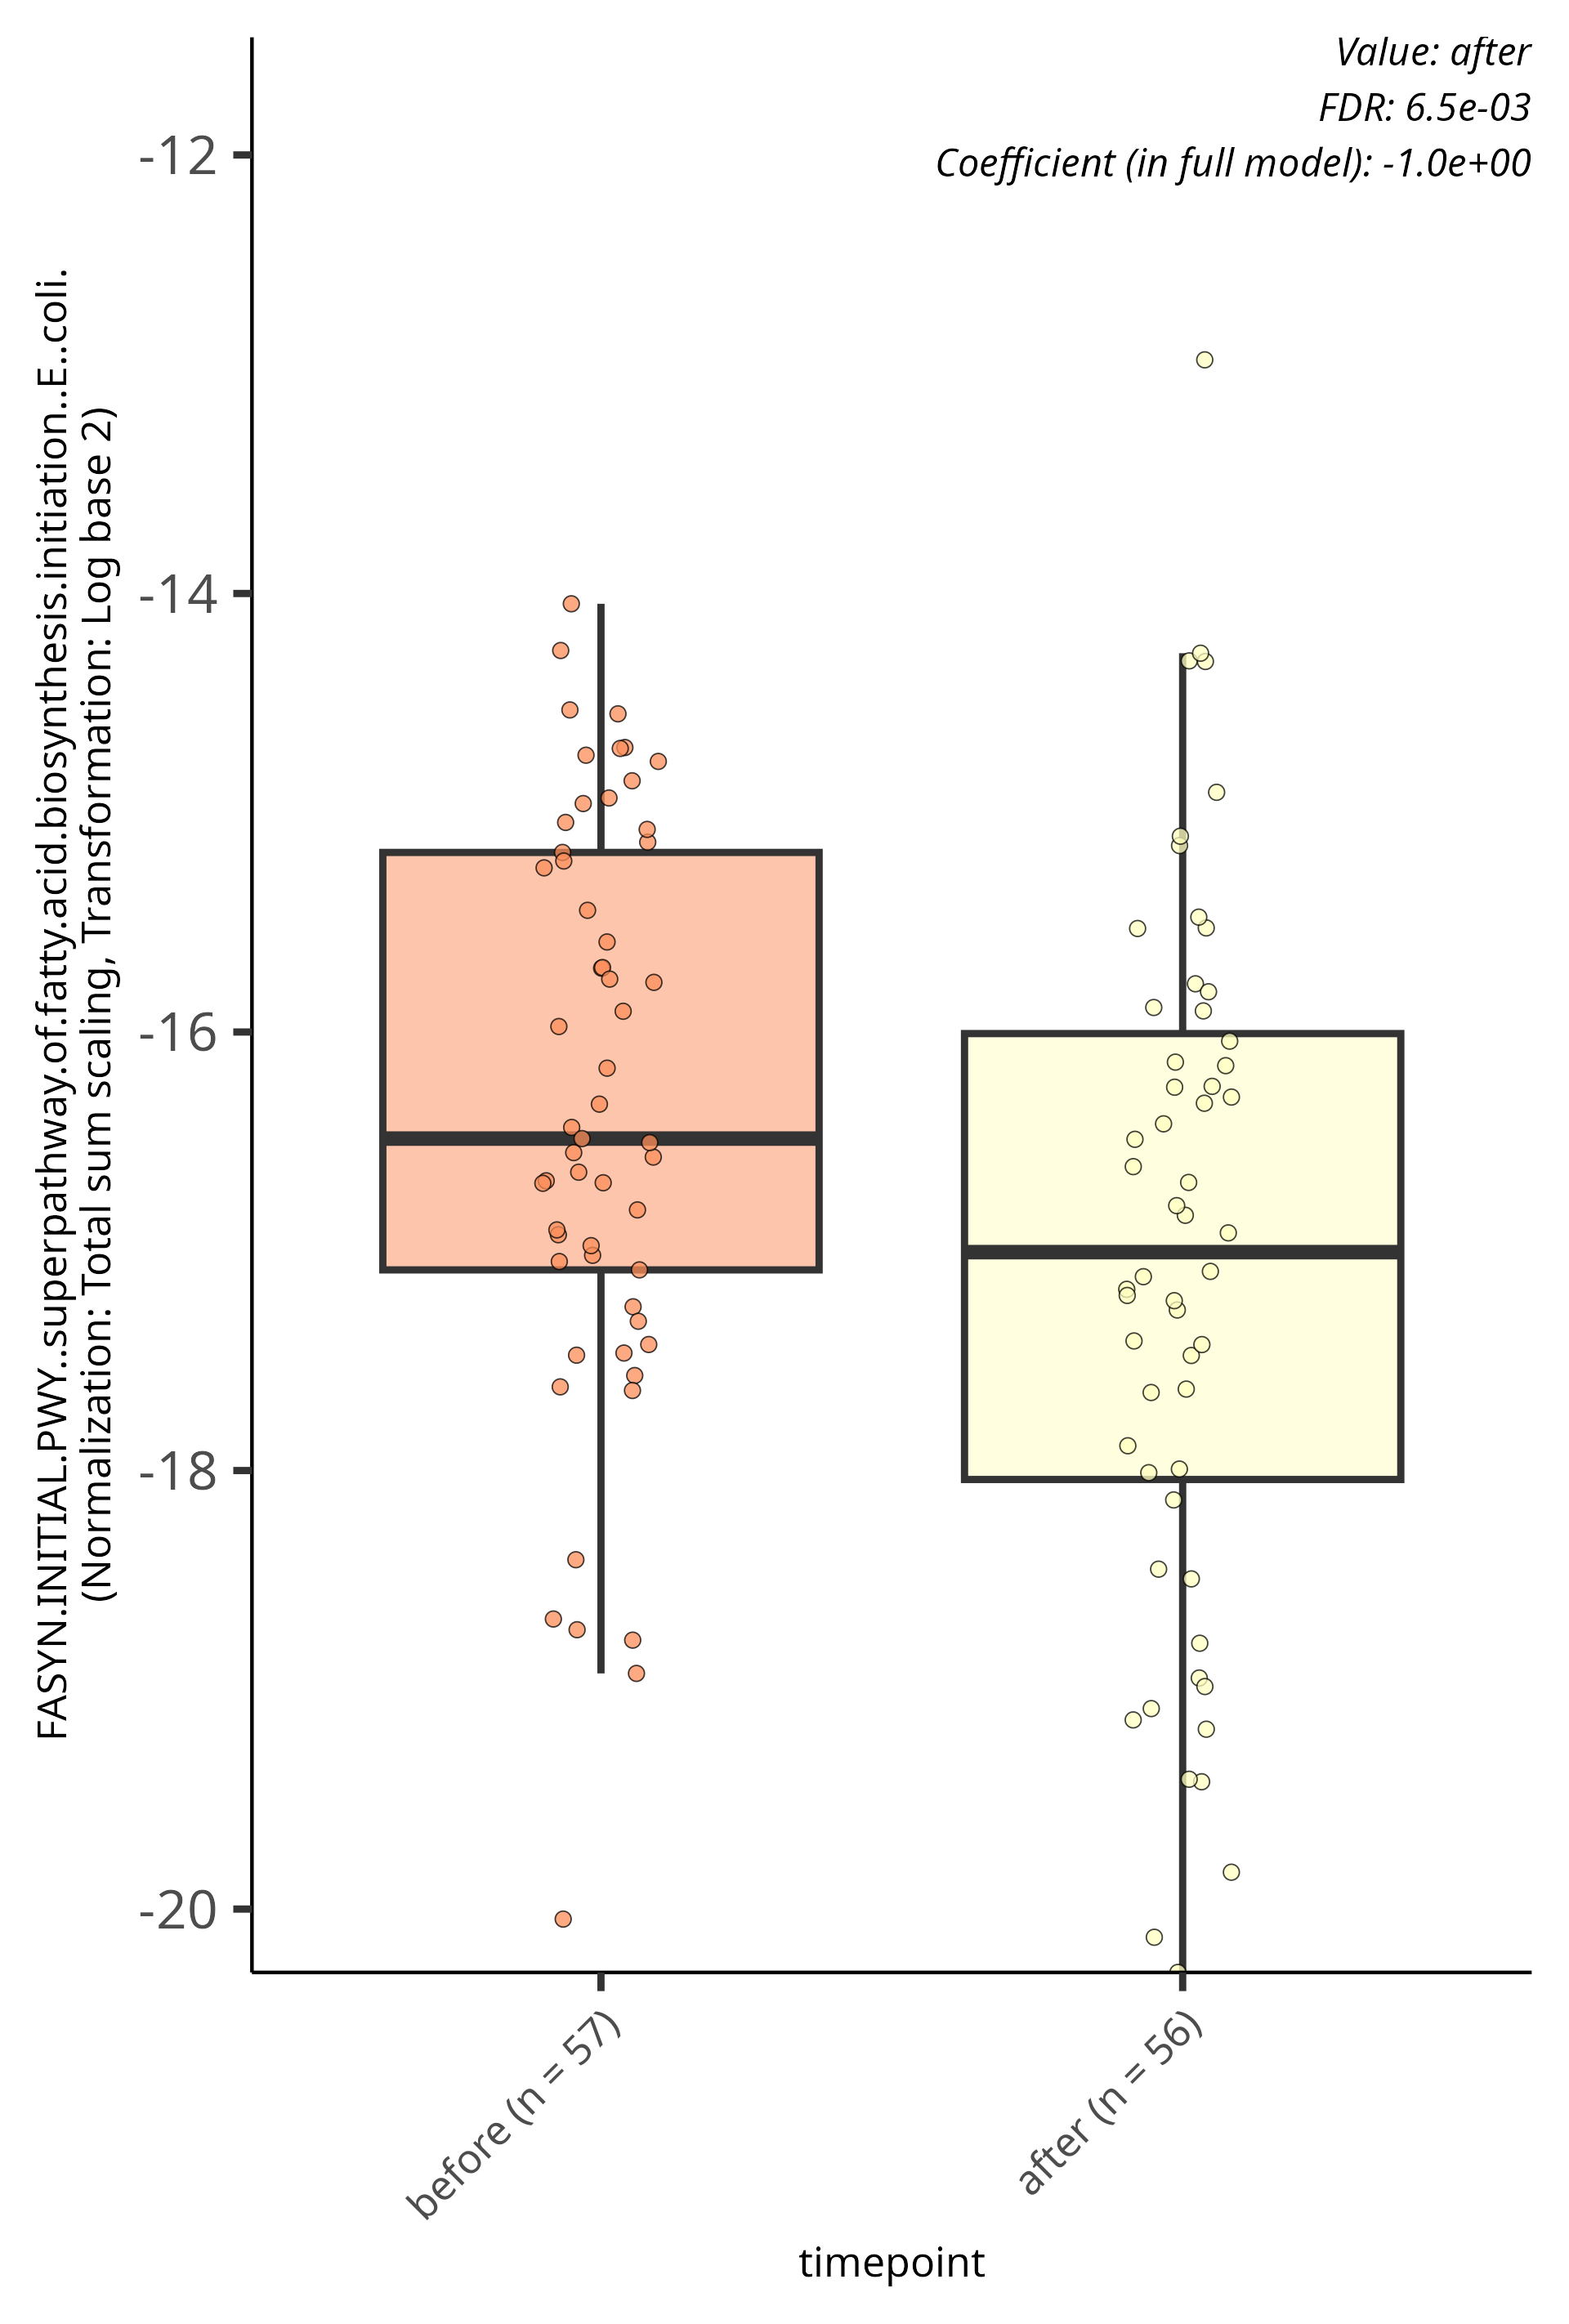
\includegraphics{../../output/daa/daa_pa/figures/association_plots/timepoint/linear/timepoint_FASYN.INITIAL.PWY..superpathway.of.fatty.acid.biosynthesis.initiation..E..coli._linear.png} \\
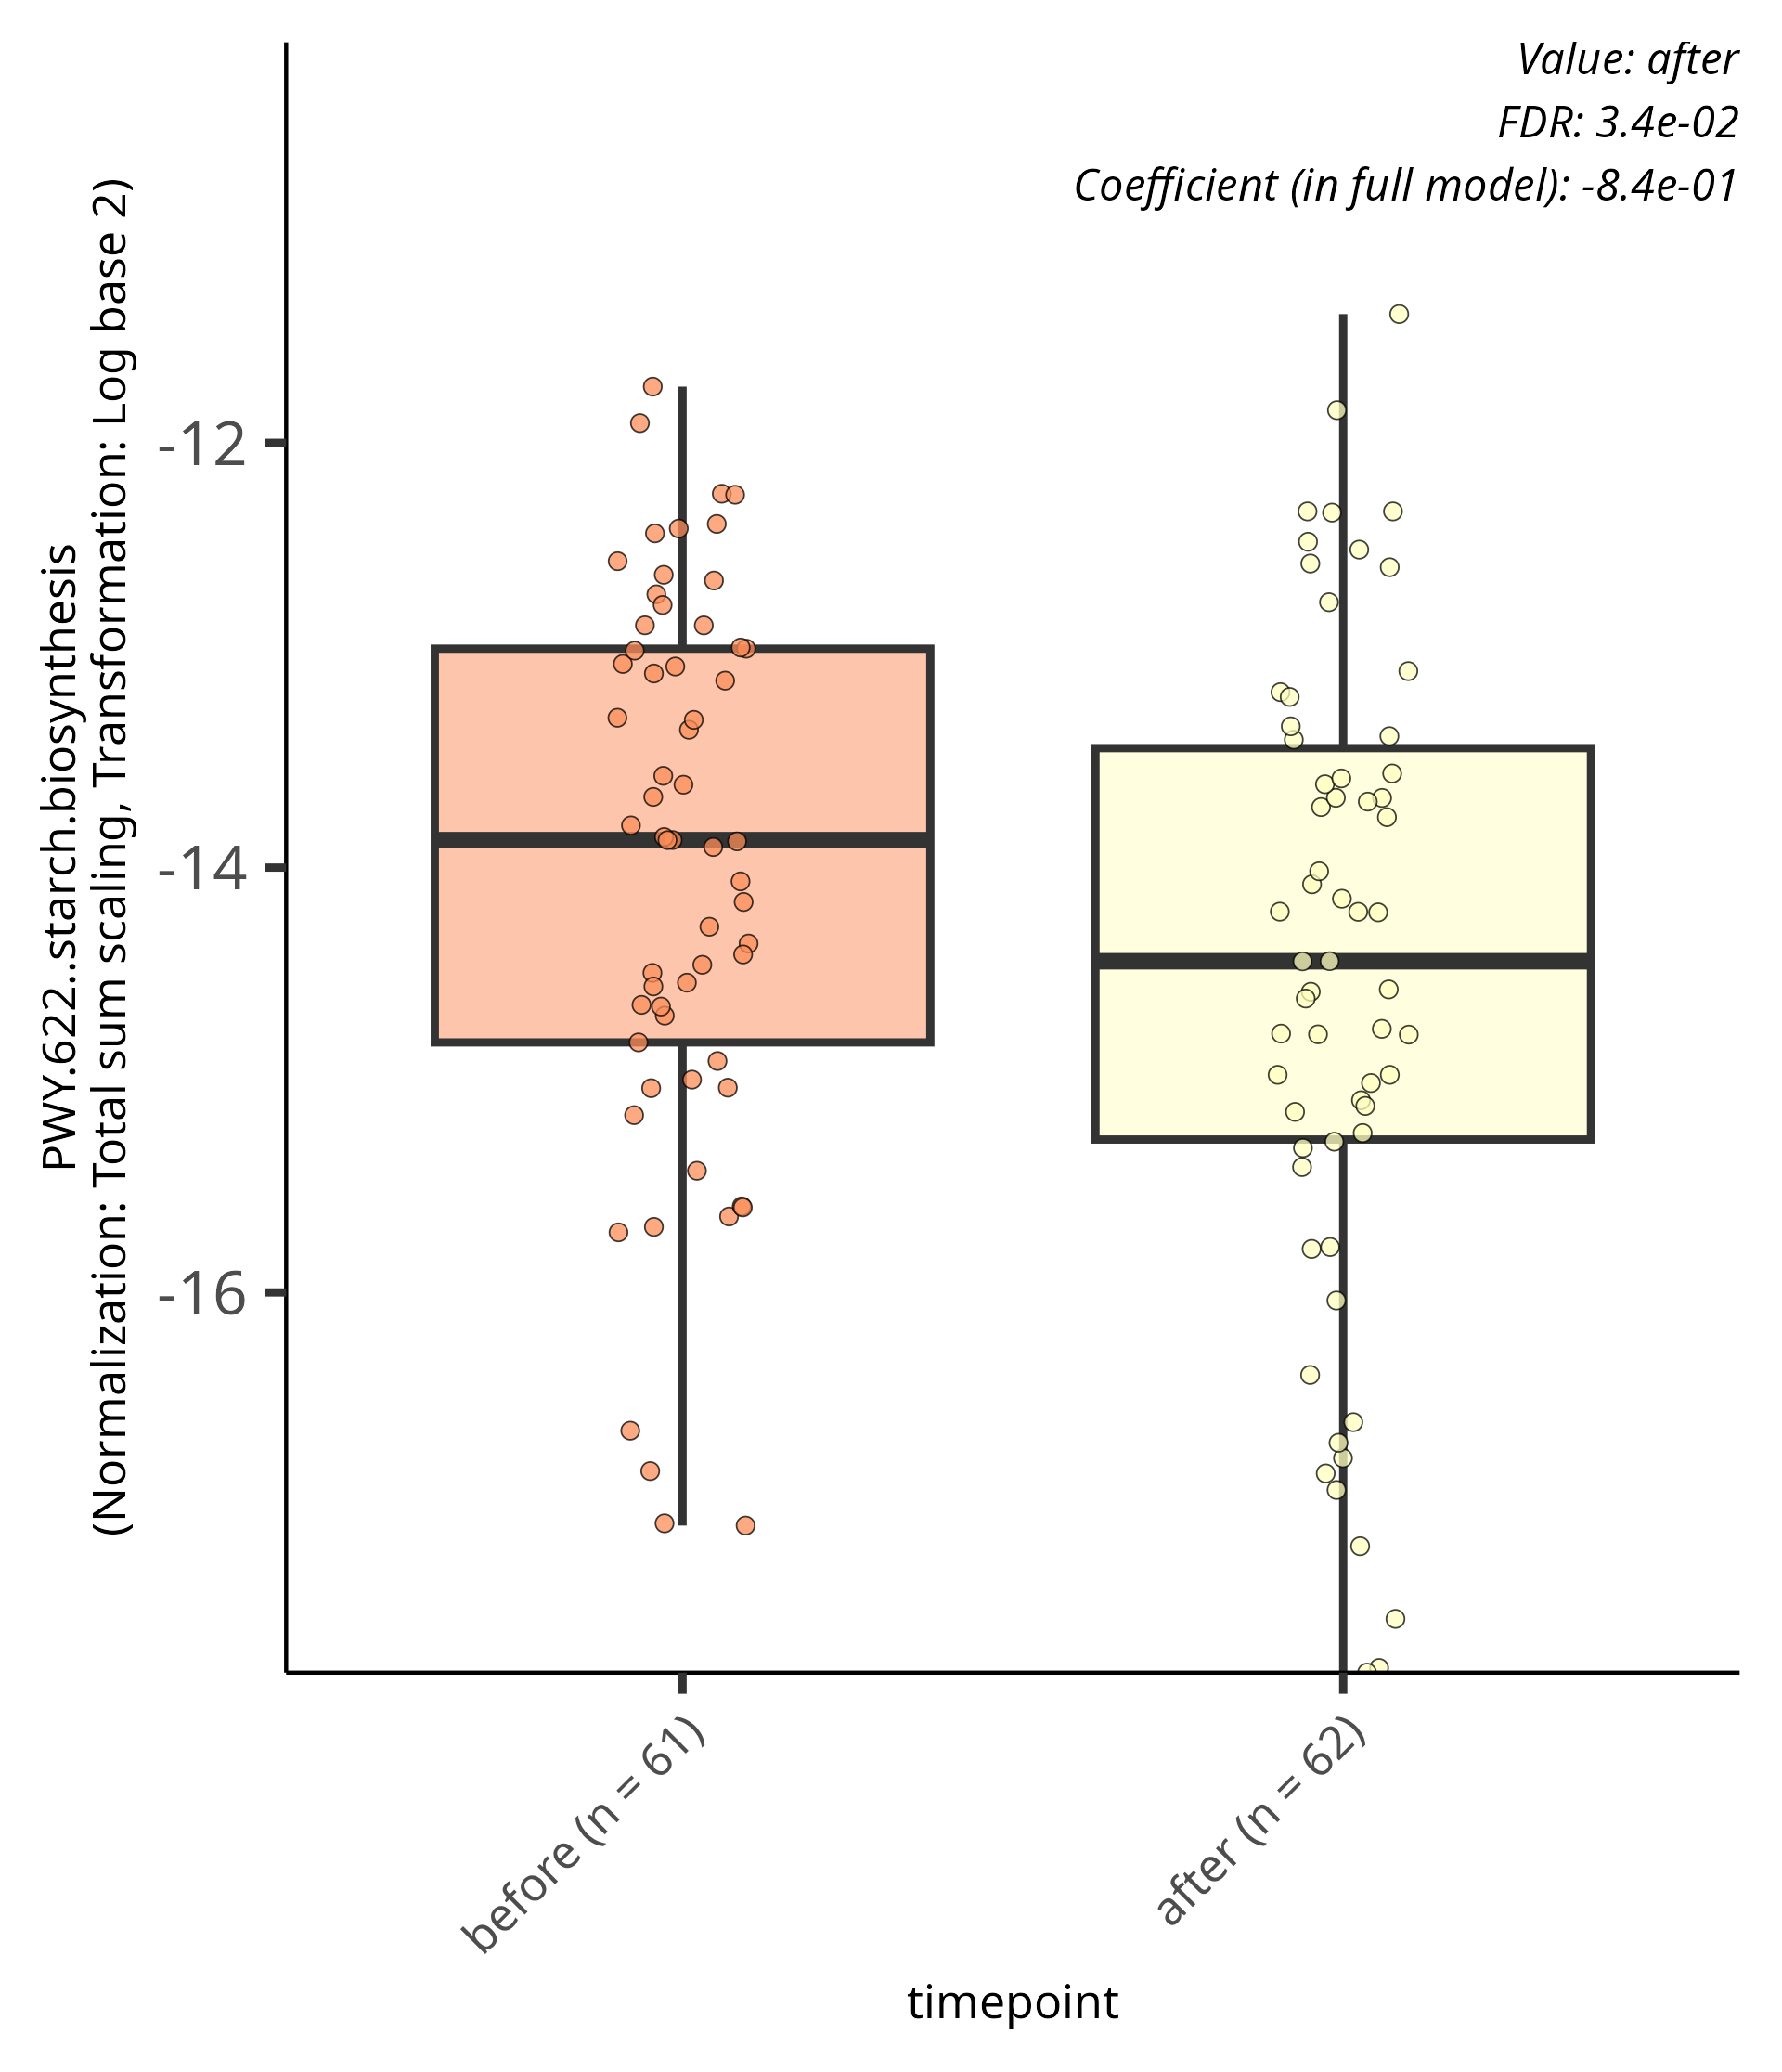
\includegraphics{../../output/daa/daa_pa/figures/association_plots/timepoint/linear/timepoint_PWY.622..starch.biosynthesis_linear.png}
&
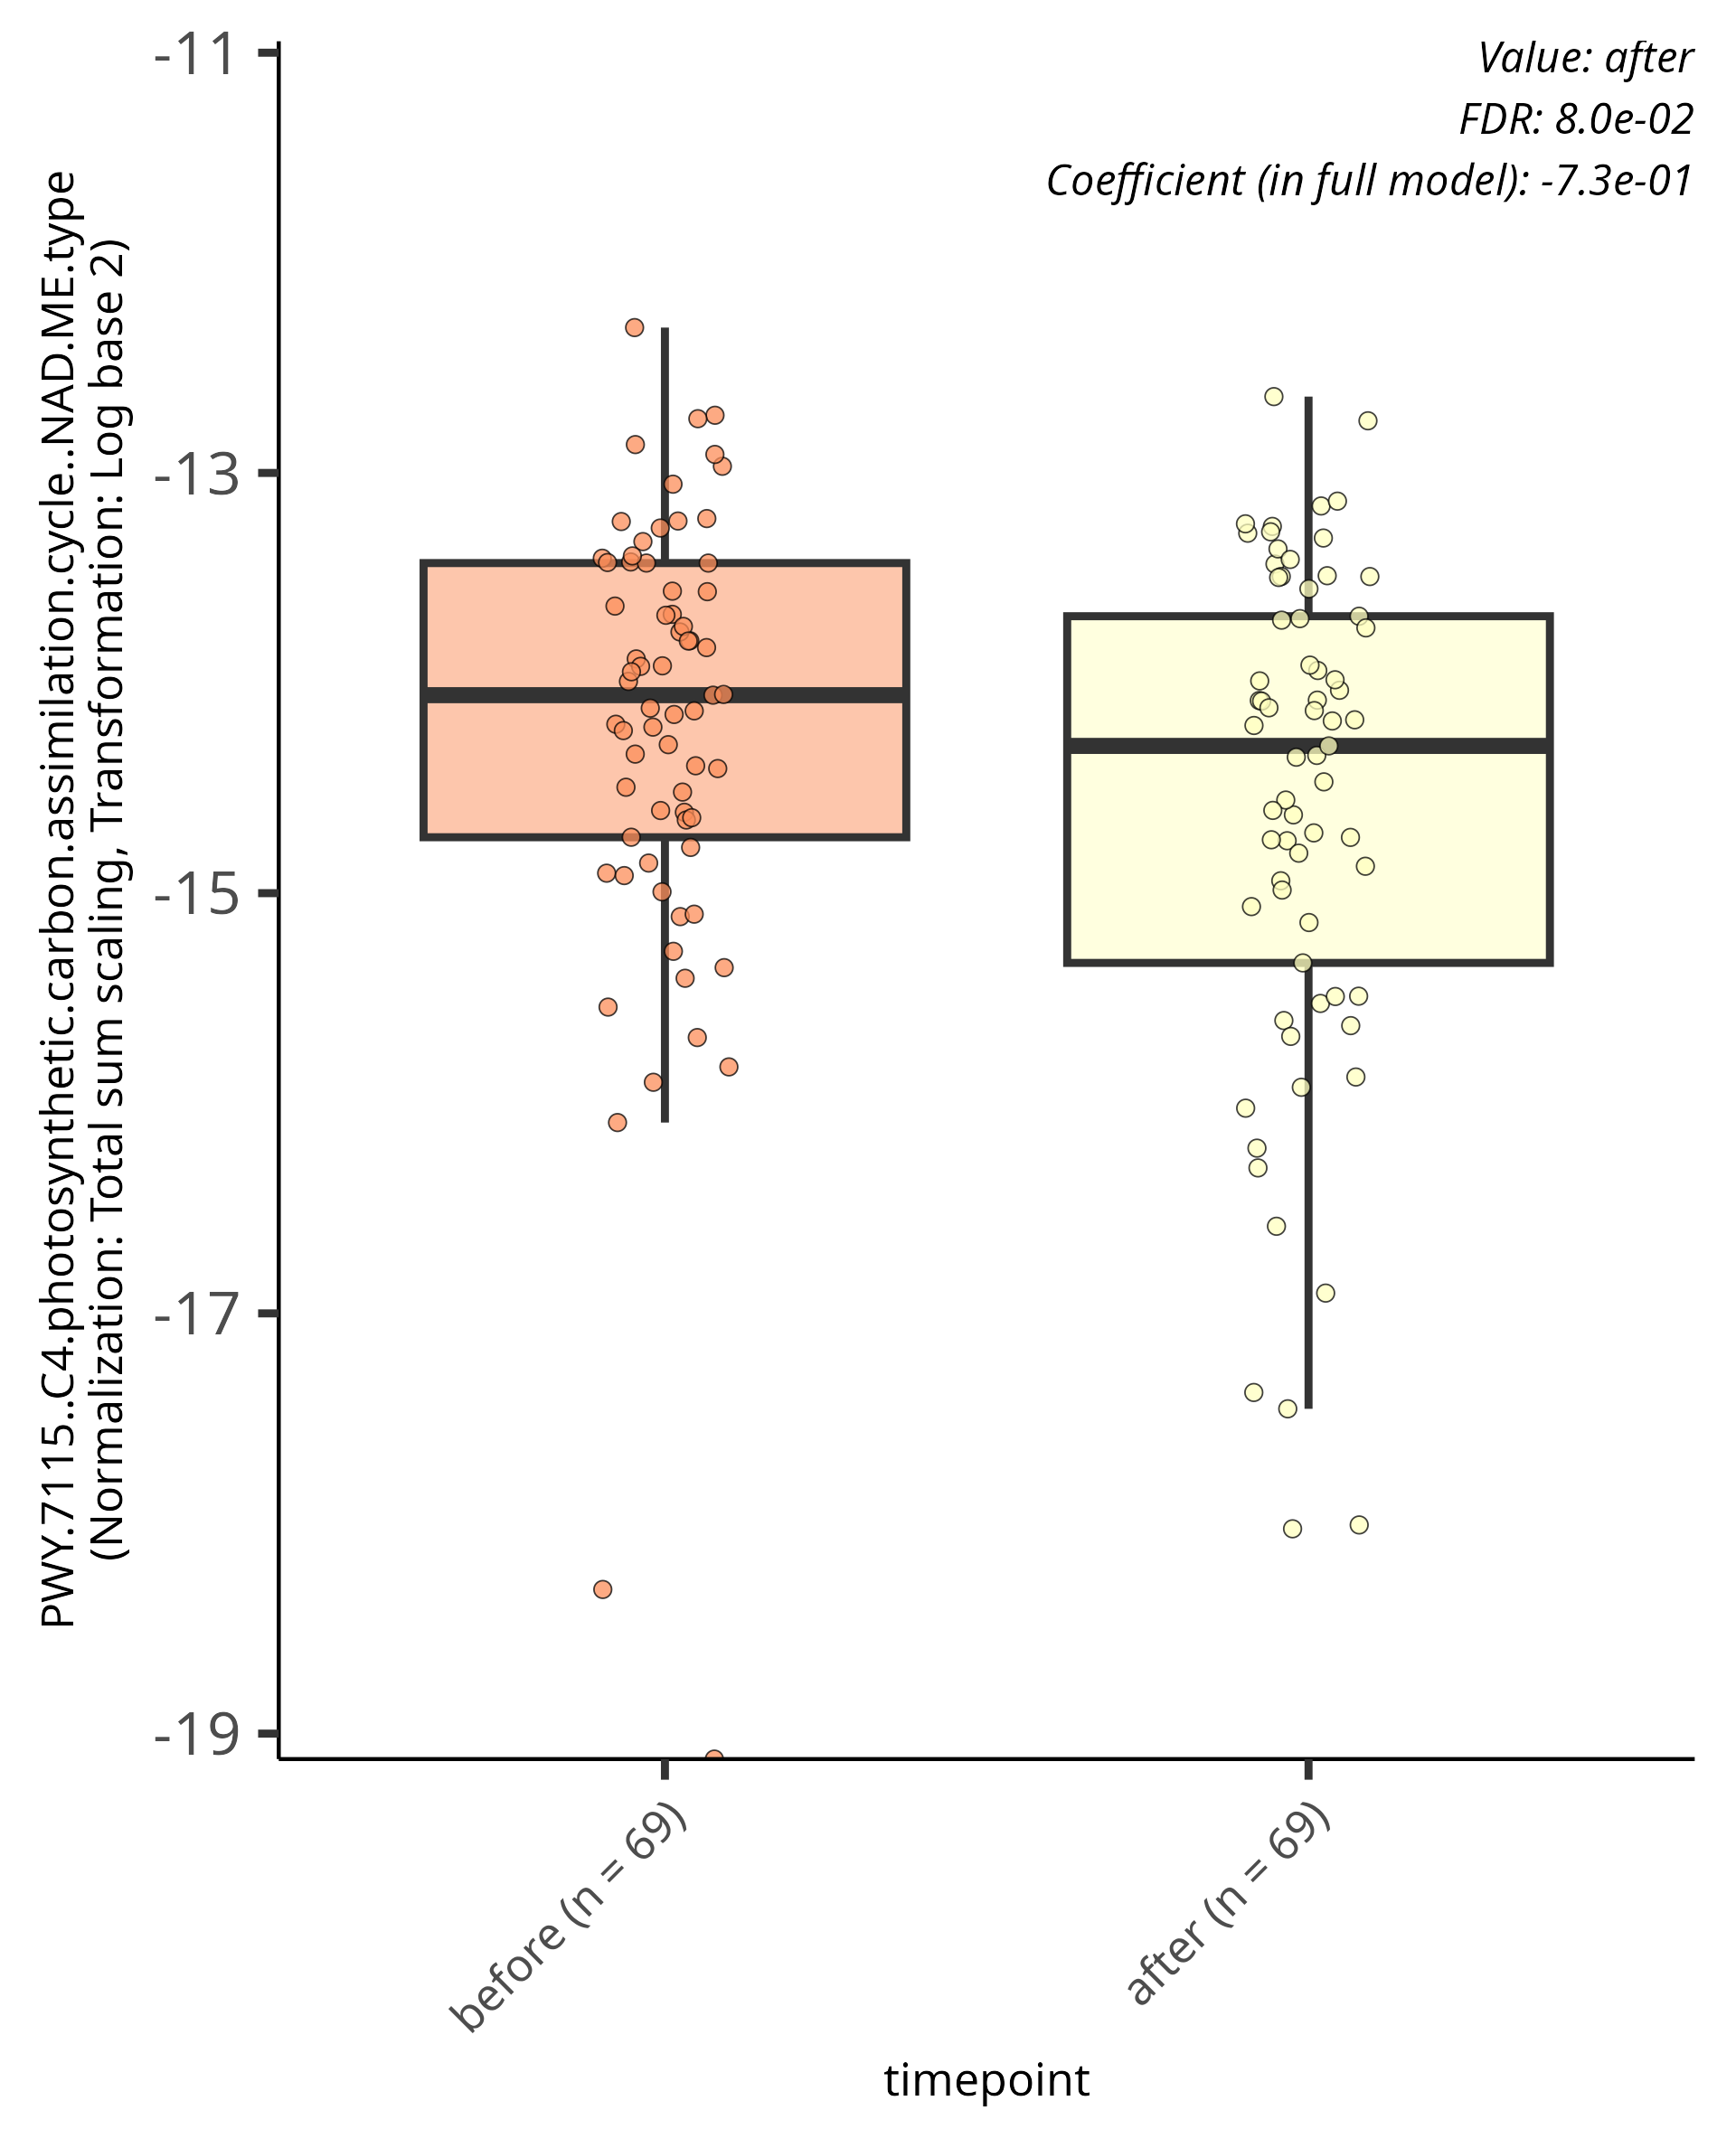
\includegraphics{../../output/daa/daa_pa/figures/association_plots/timepoint/linear/timepoint_PWY.7115..C4.photosynthetic.carbon.assimilation.cycle..NAD.ME.type_linear.png}
&
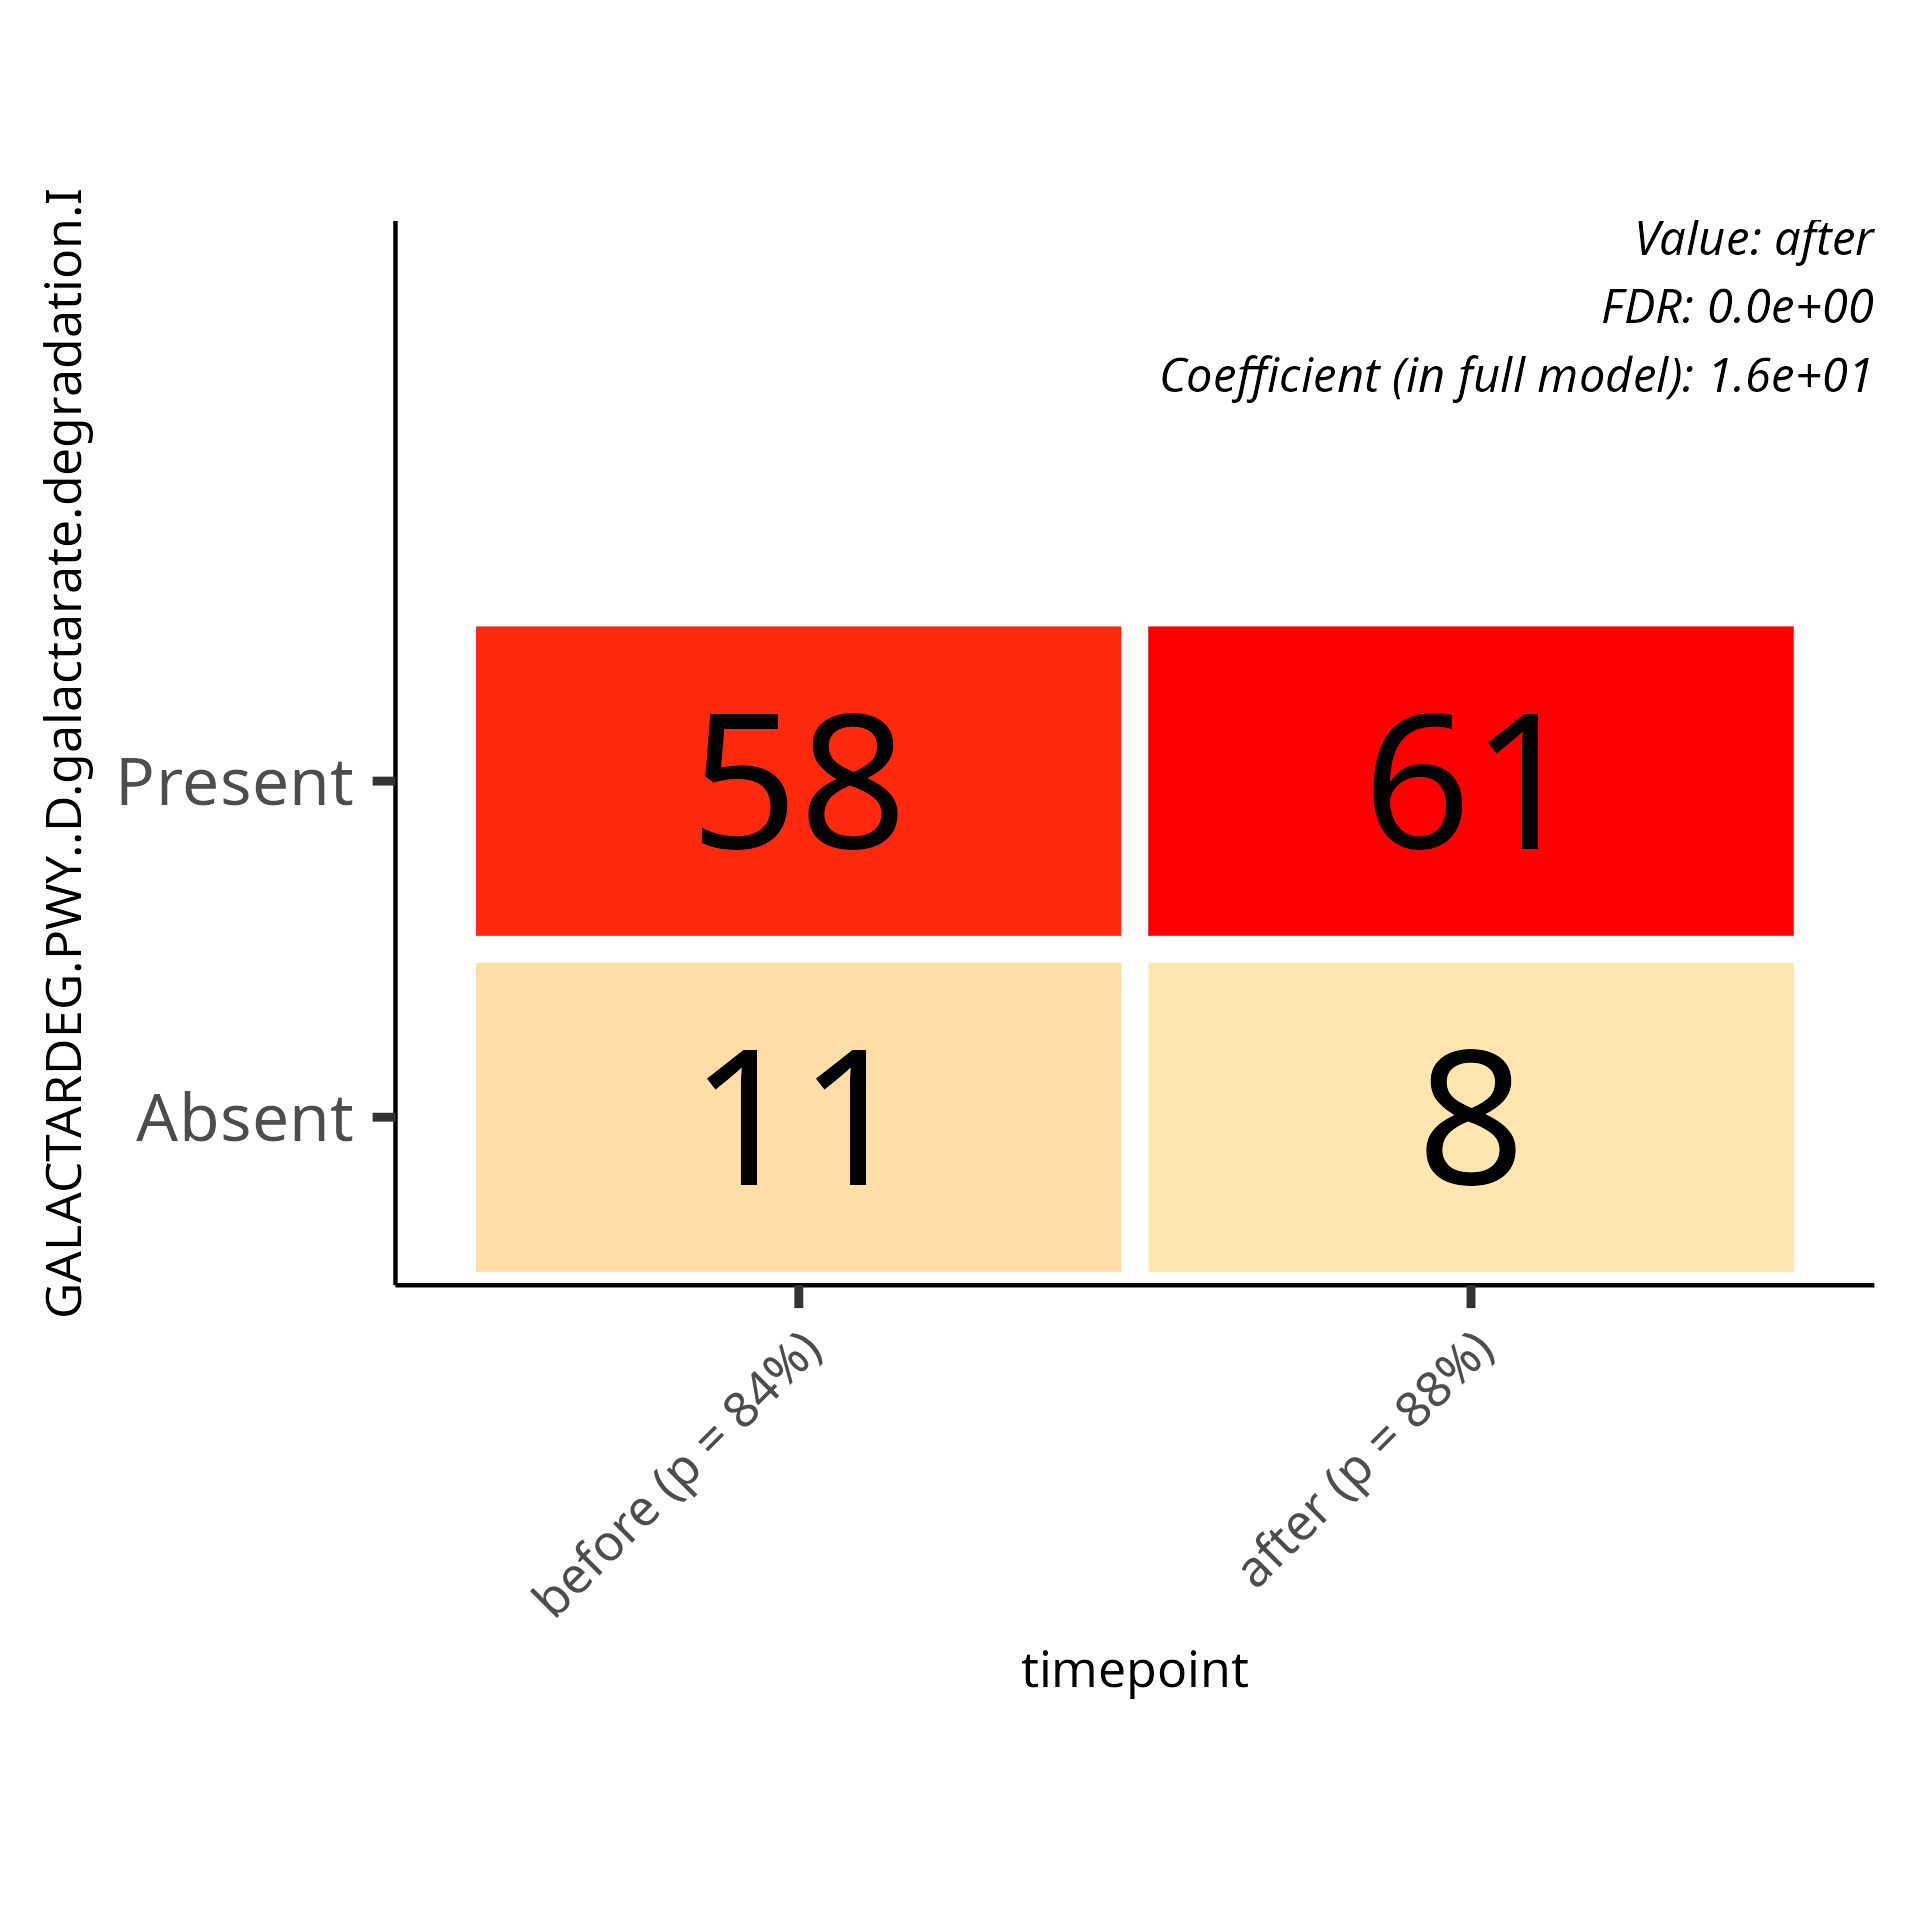
\includegraphics{../../output/daa/daa_pa/figures/association_plots/timepoint/logistic/timepoint_GALACTARDEG.PWY..D.galactarate.degradation.I_logistic.png}
&
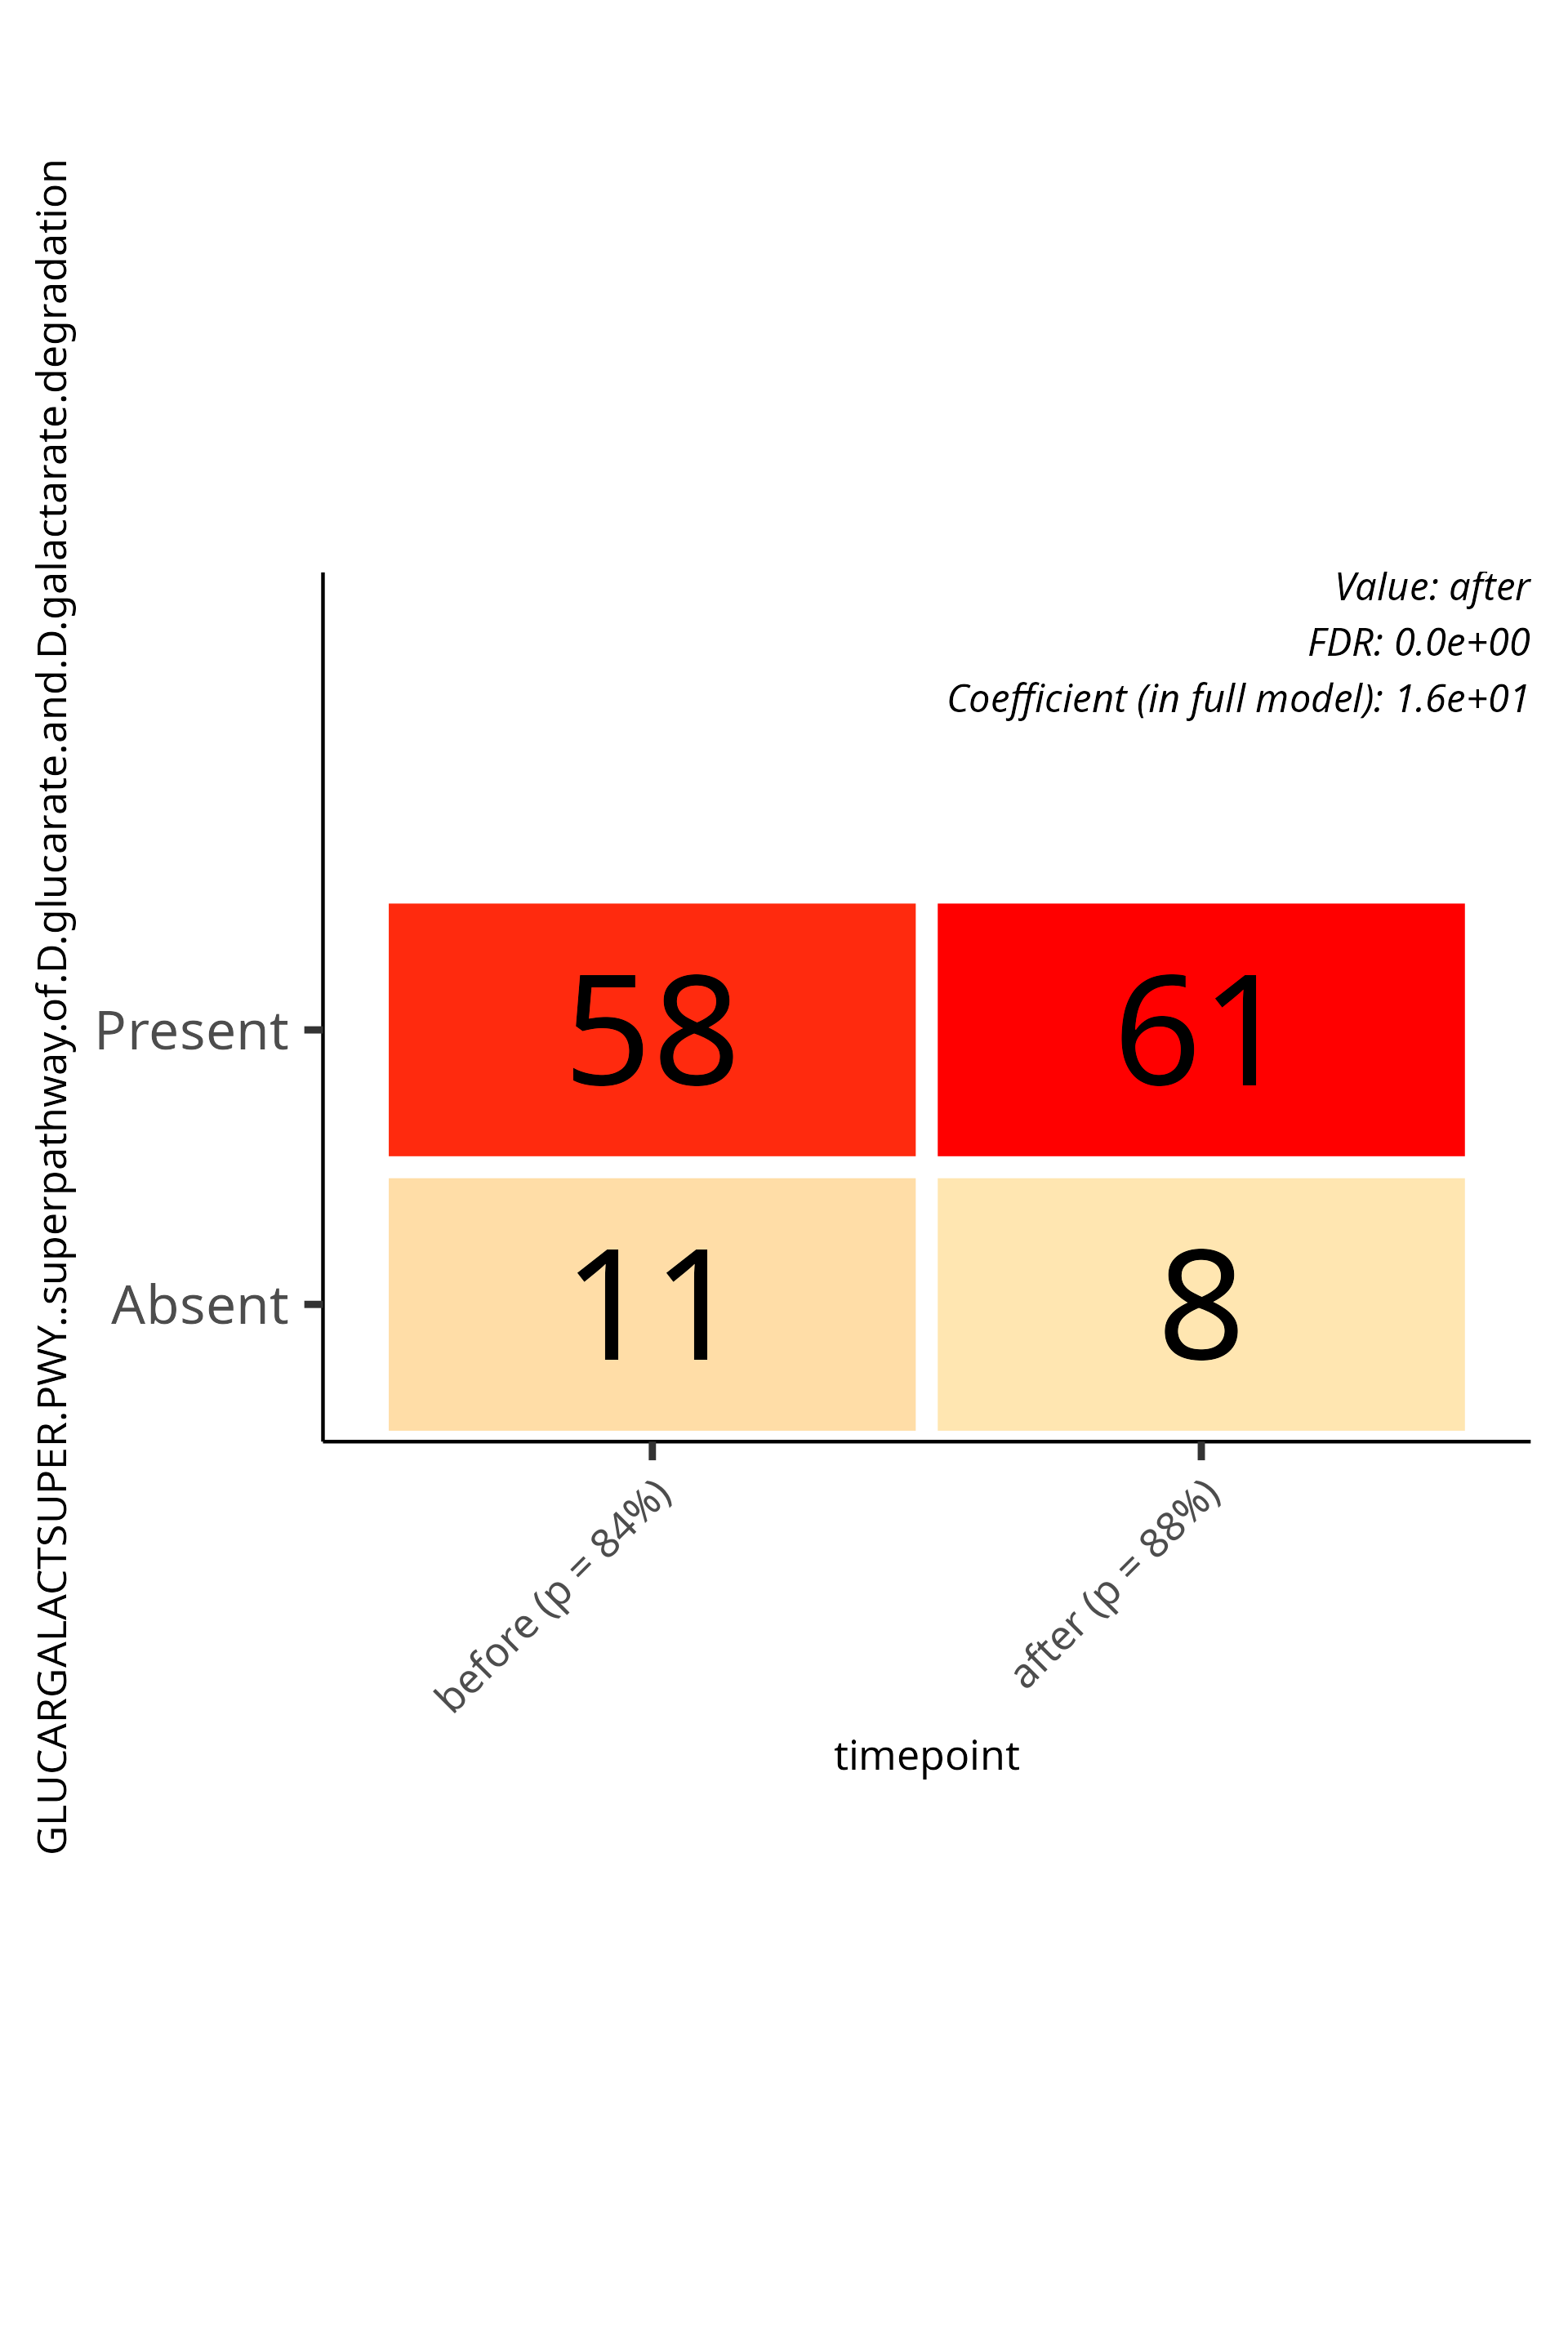
\includegraphics{../../output/daa/daa_pa/figures/association_plots/timepoint/logistic/timepoint_GLUCARGALACTSUPER.PWY..superpathway.of.D.glucarate.and.D.galactarate.degradation_logistic.png} \\
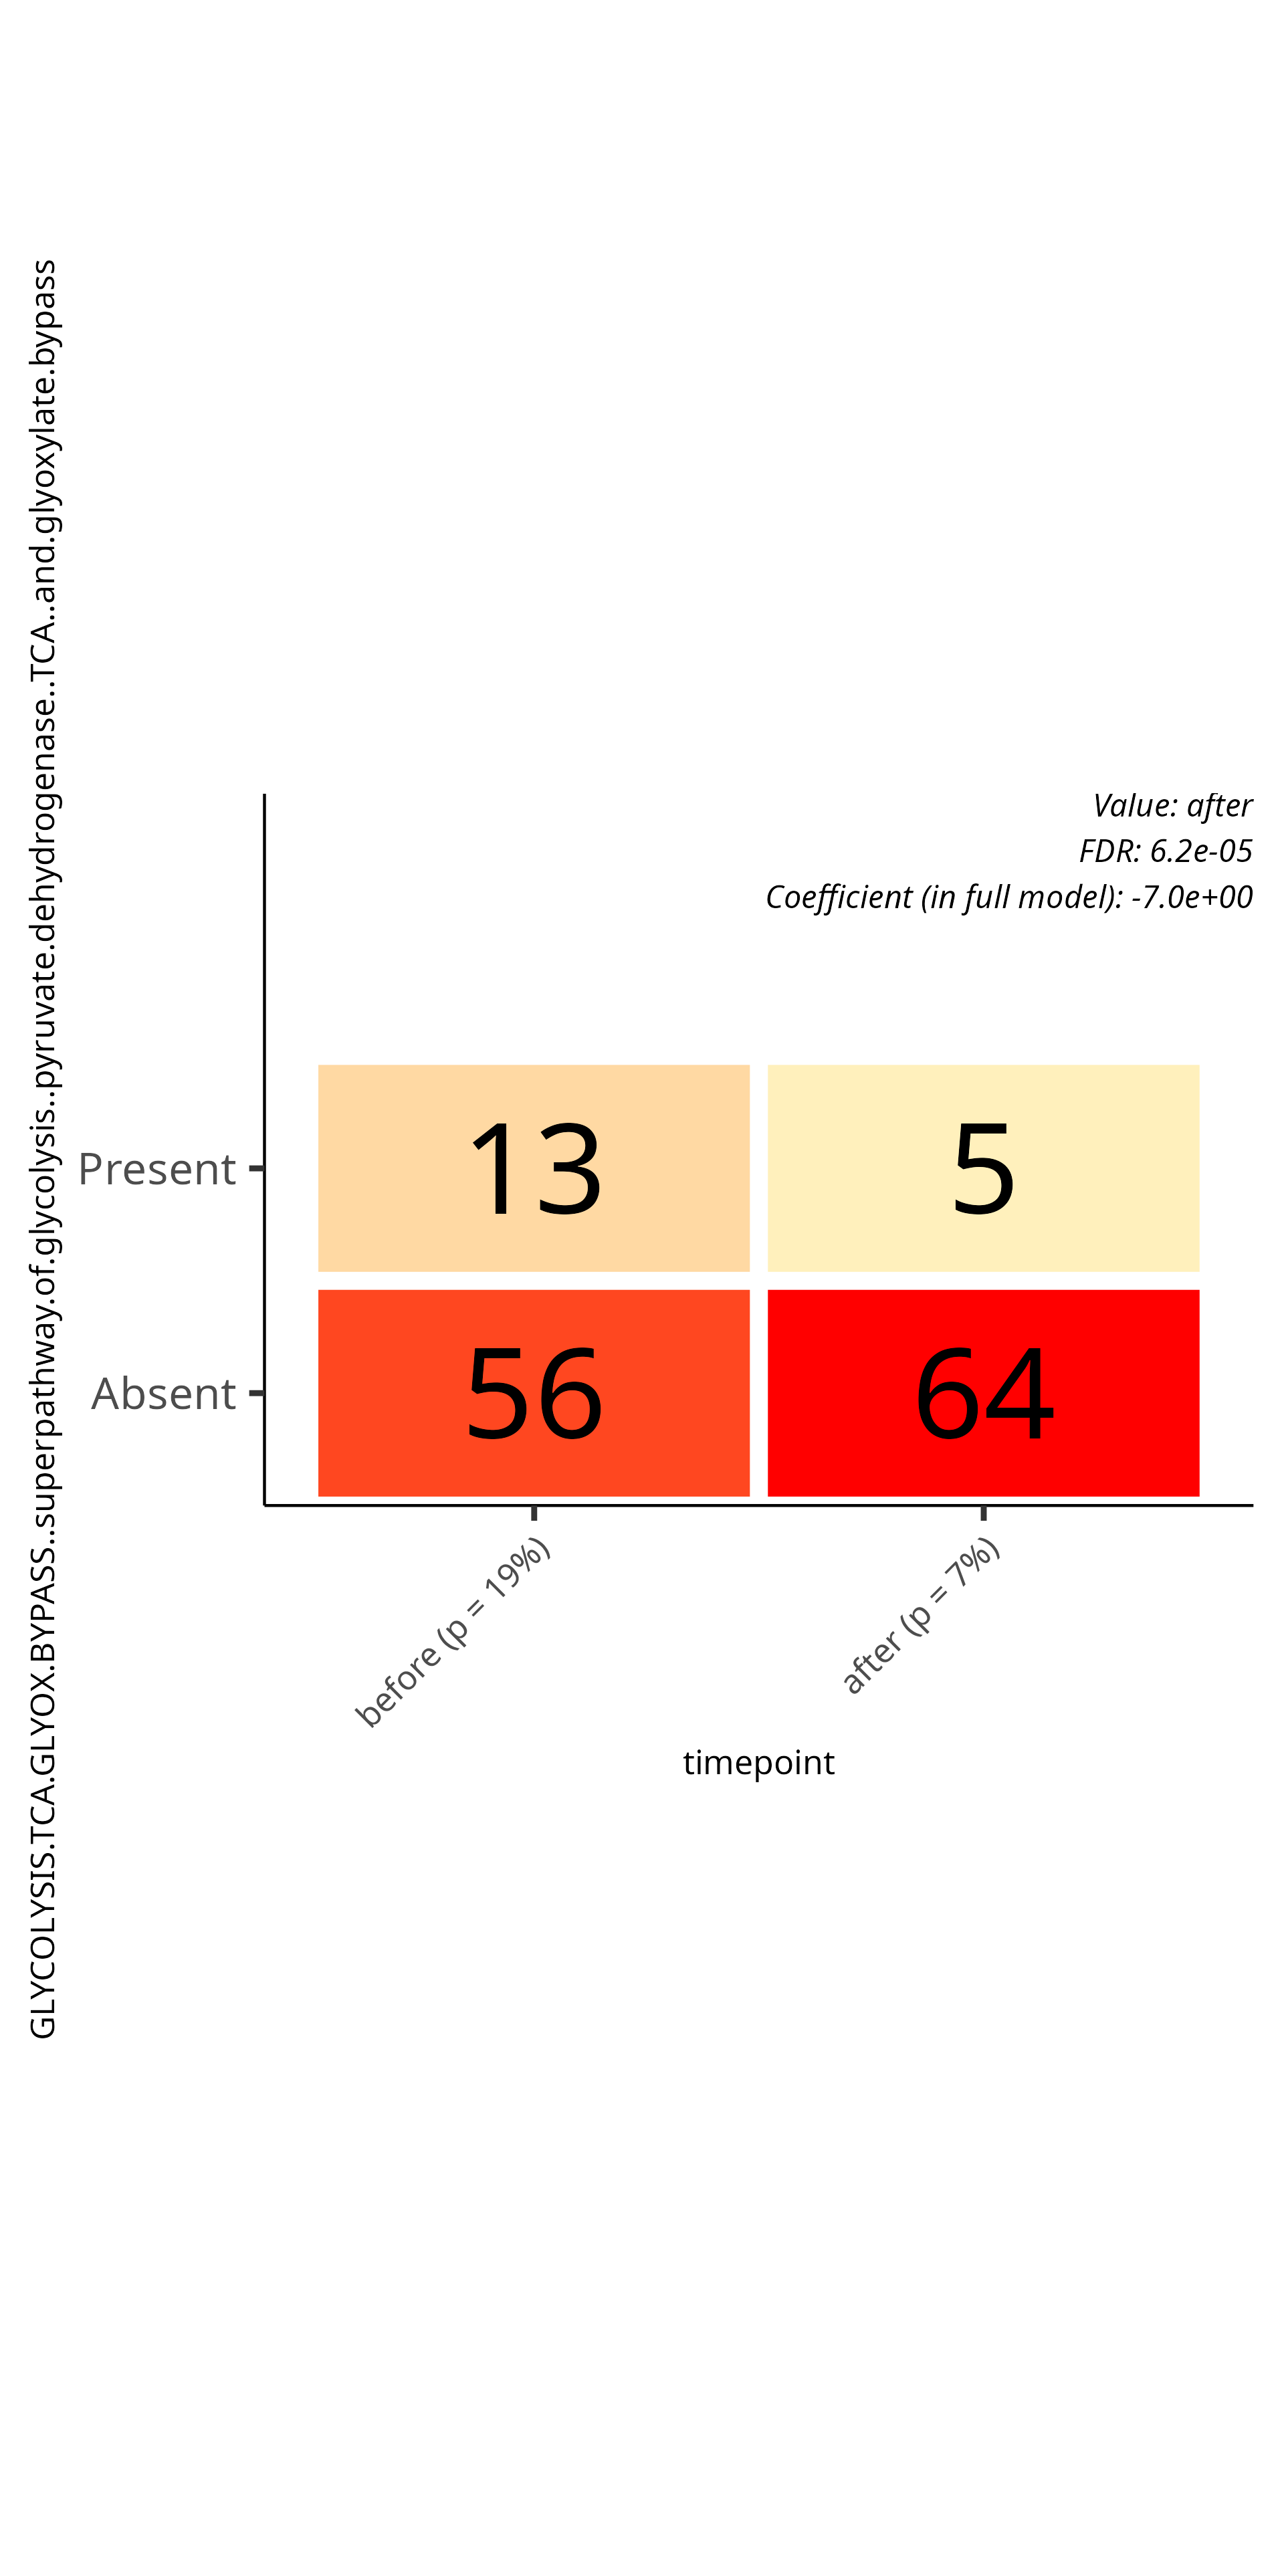
\includegraphics{../../output/daa/daa_pa/figures/association_plots/timepoint/logistic/timepoint_GLYCOLYSIS.TCA.GLYOX.BYPASS..superpathway.of.glycolysis..pyruvate.dehydrogenase..TCA..and.glyoxylate.bypass_logistic.png}
&
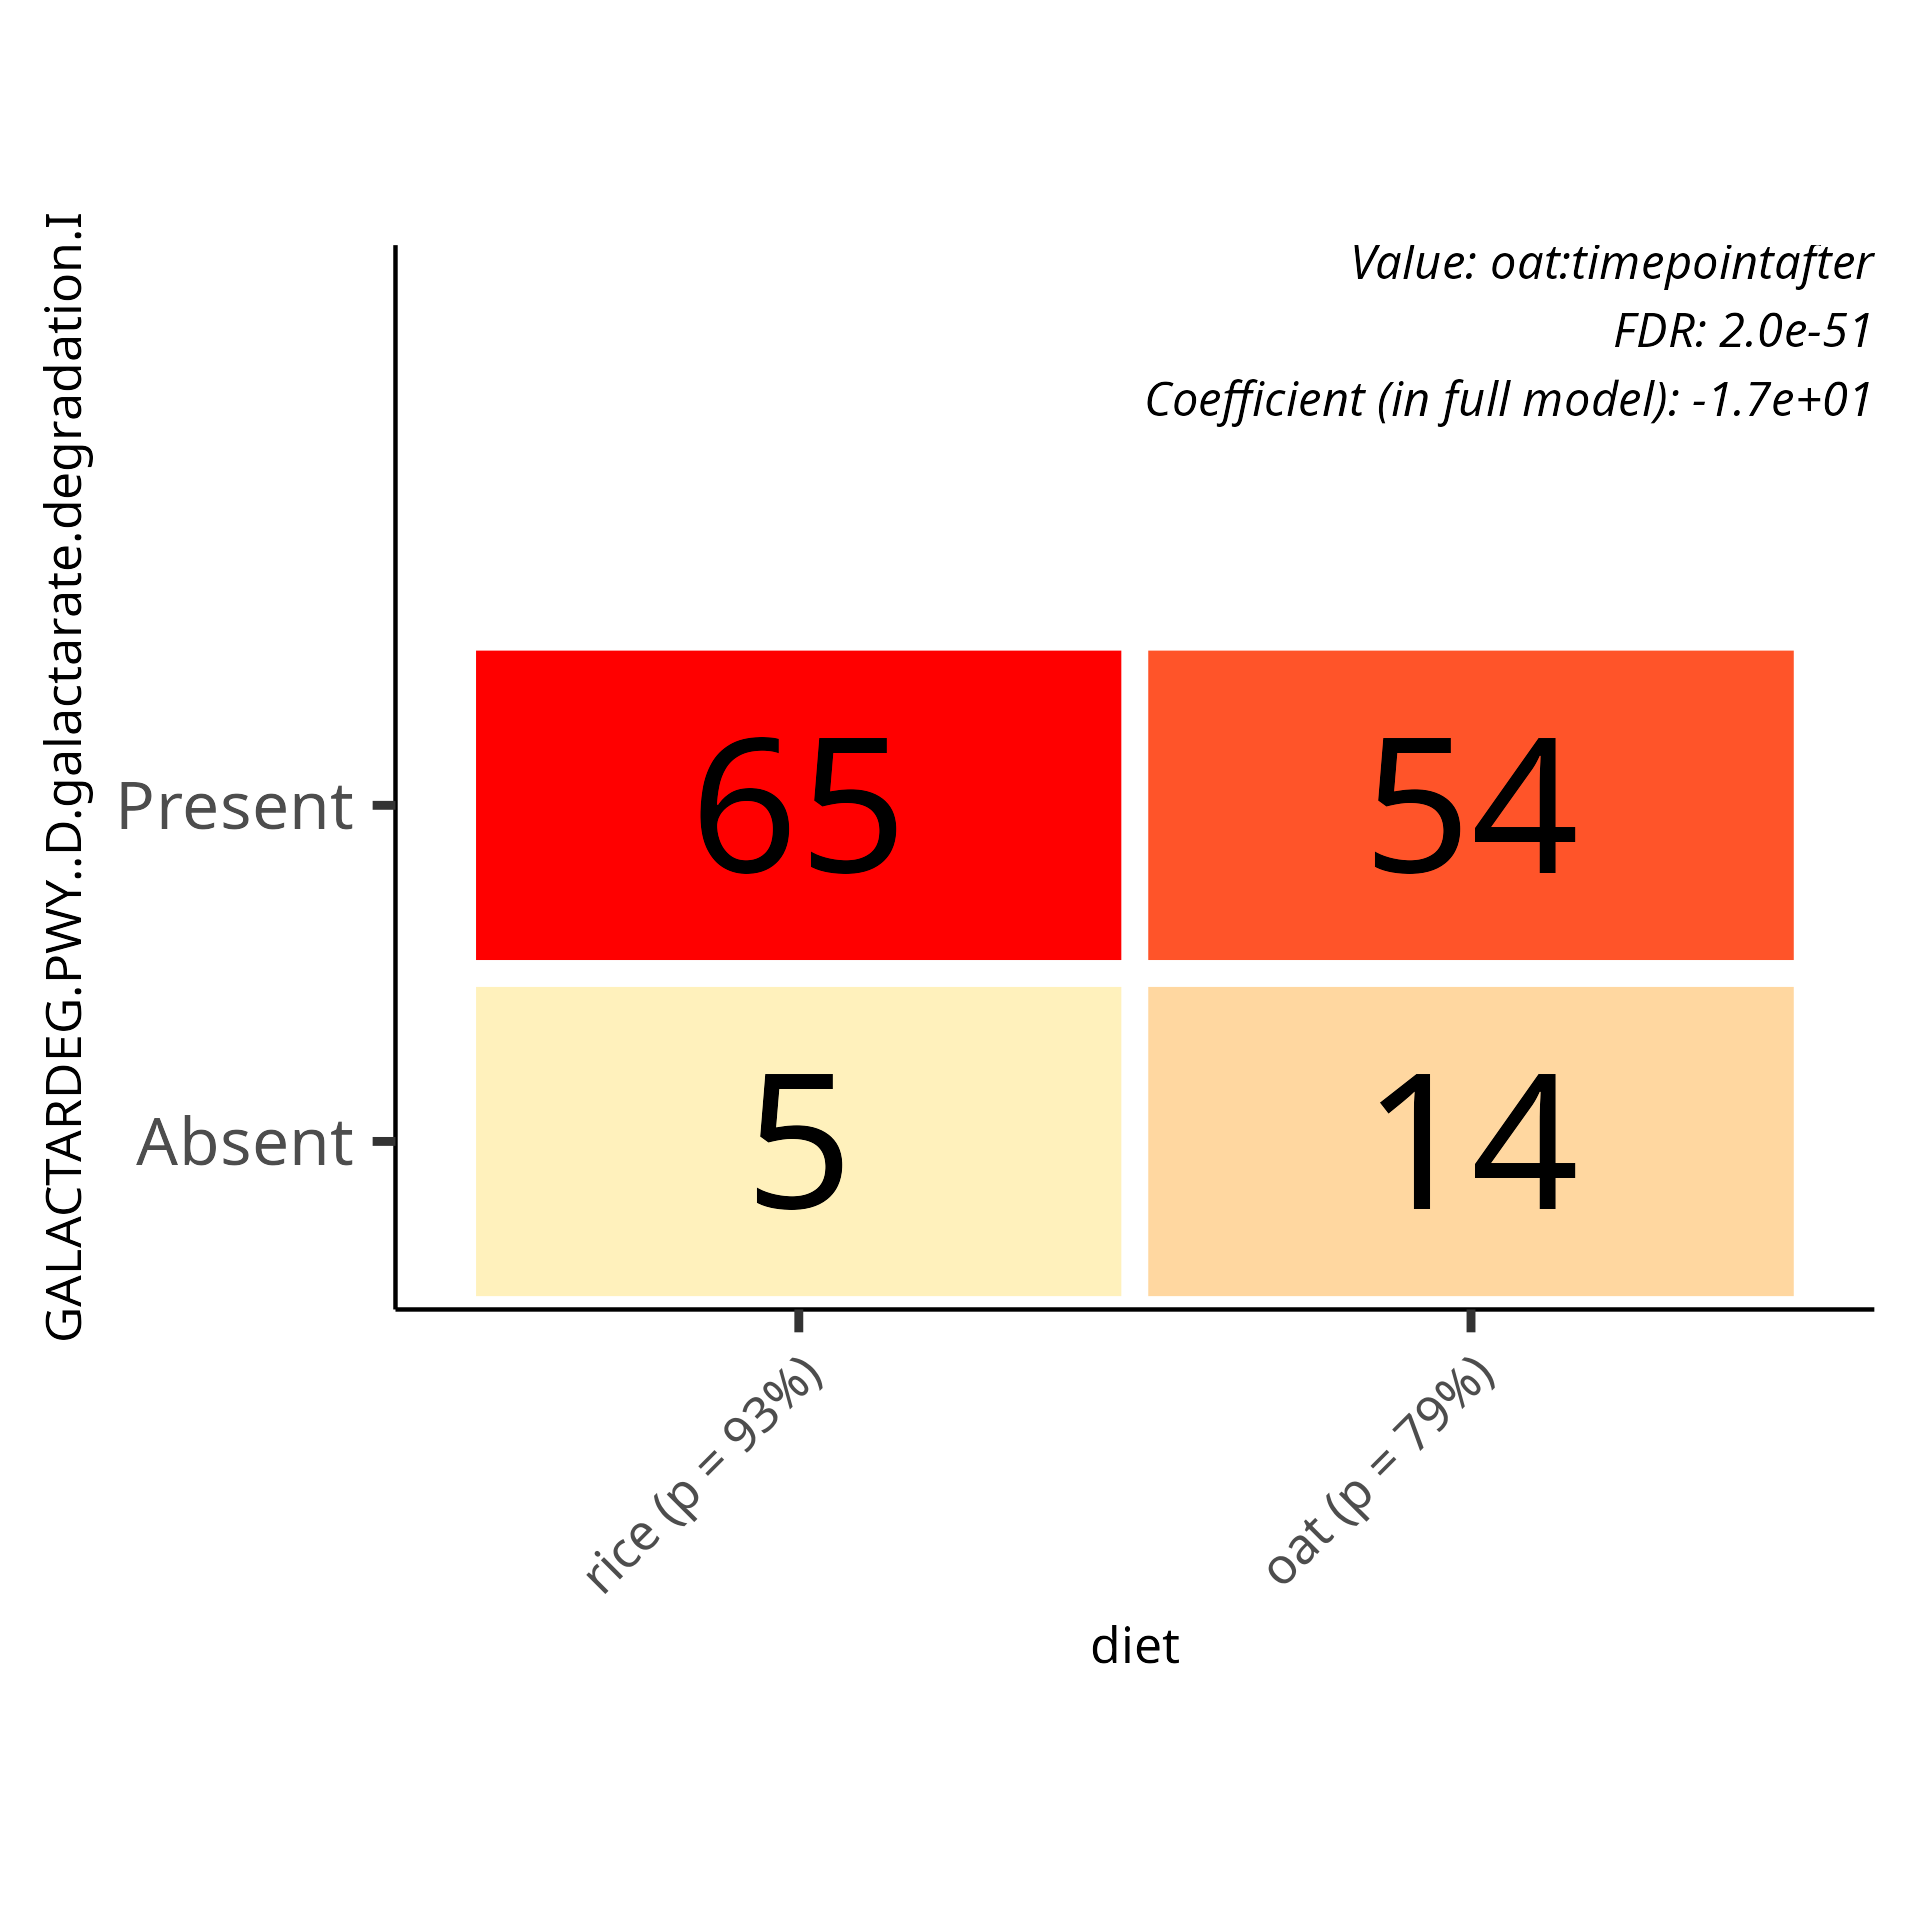
\includegraphics{../../output/daa/daa_pa/figures/association_plots/diet/logistic/diet_GALACTARDEG.PWY..D.galactarate.degradation.I_logistic.png}
&
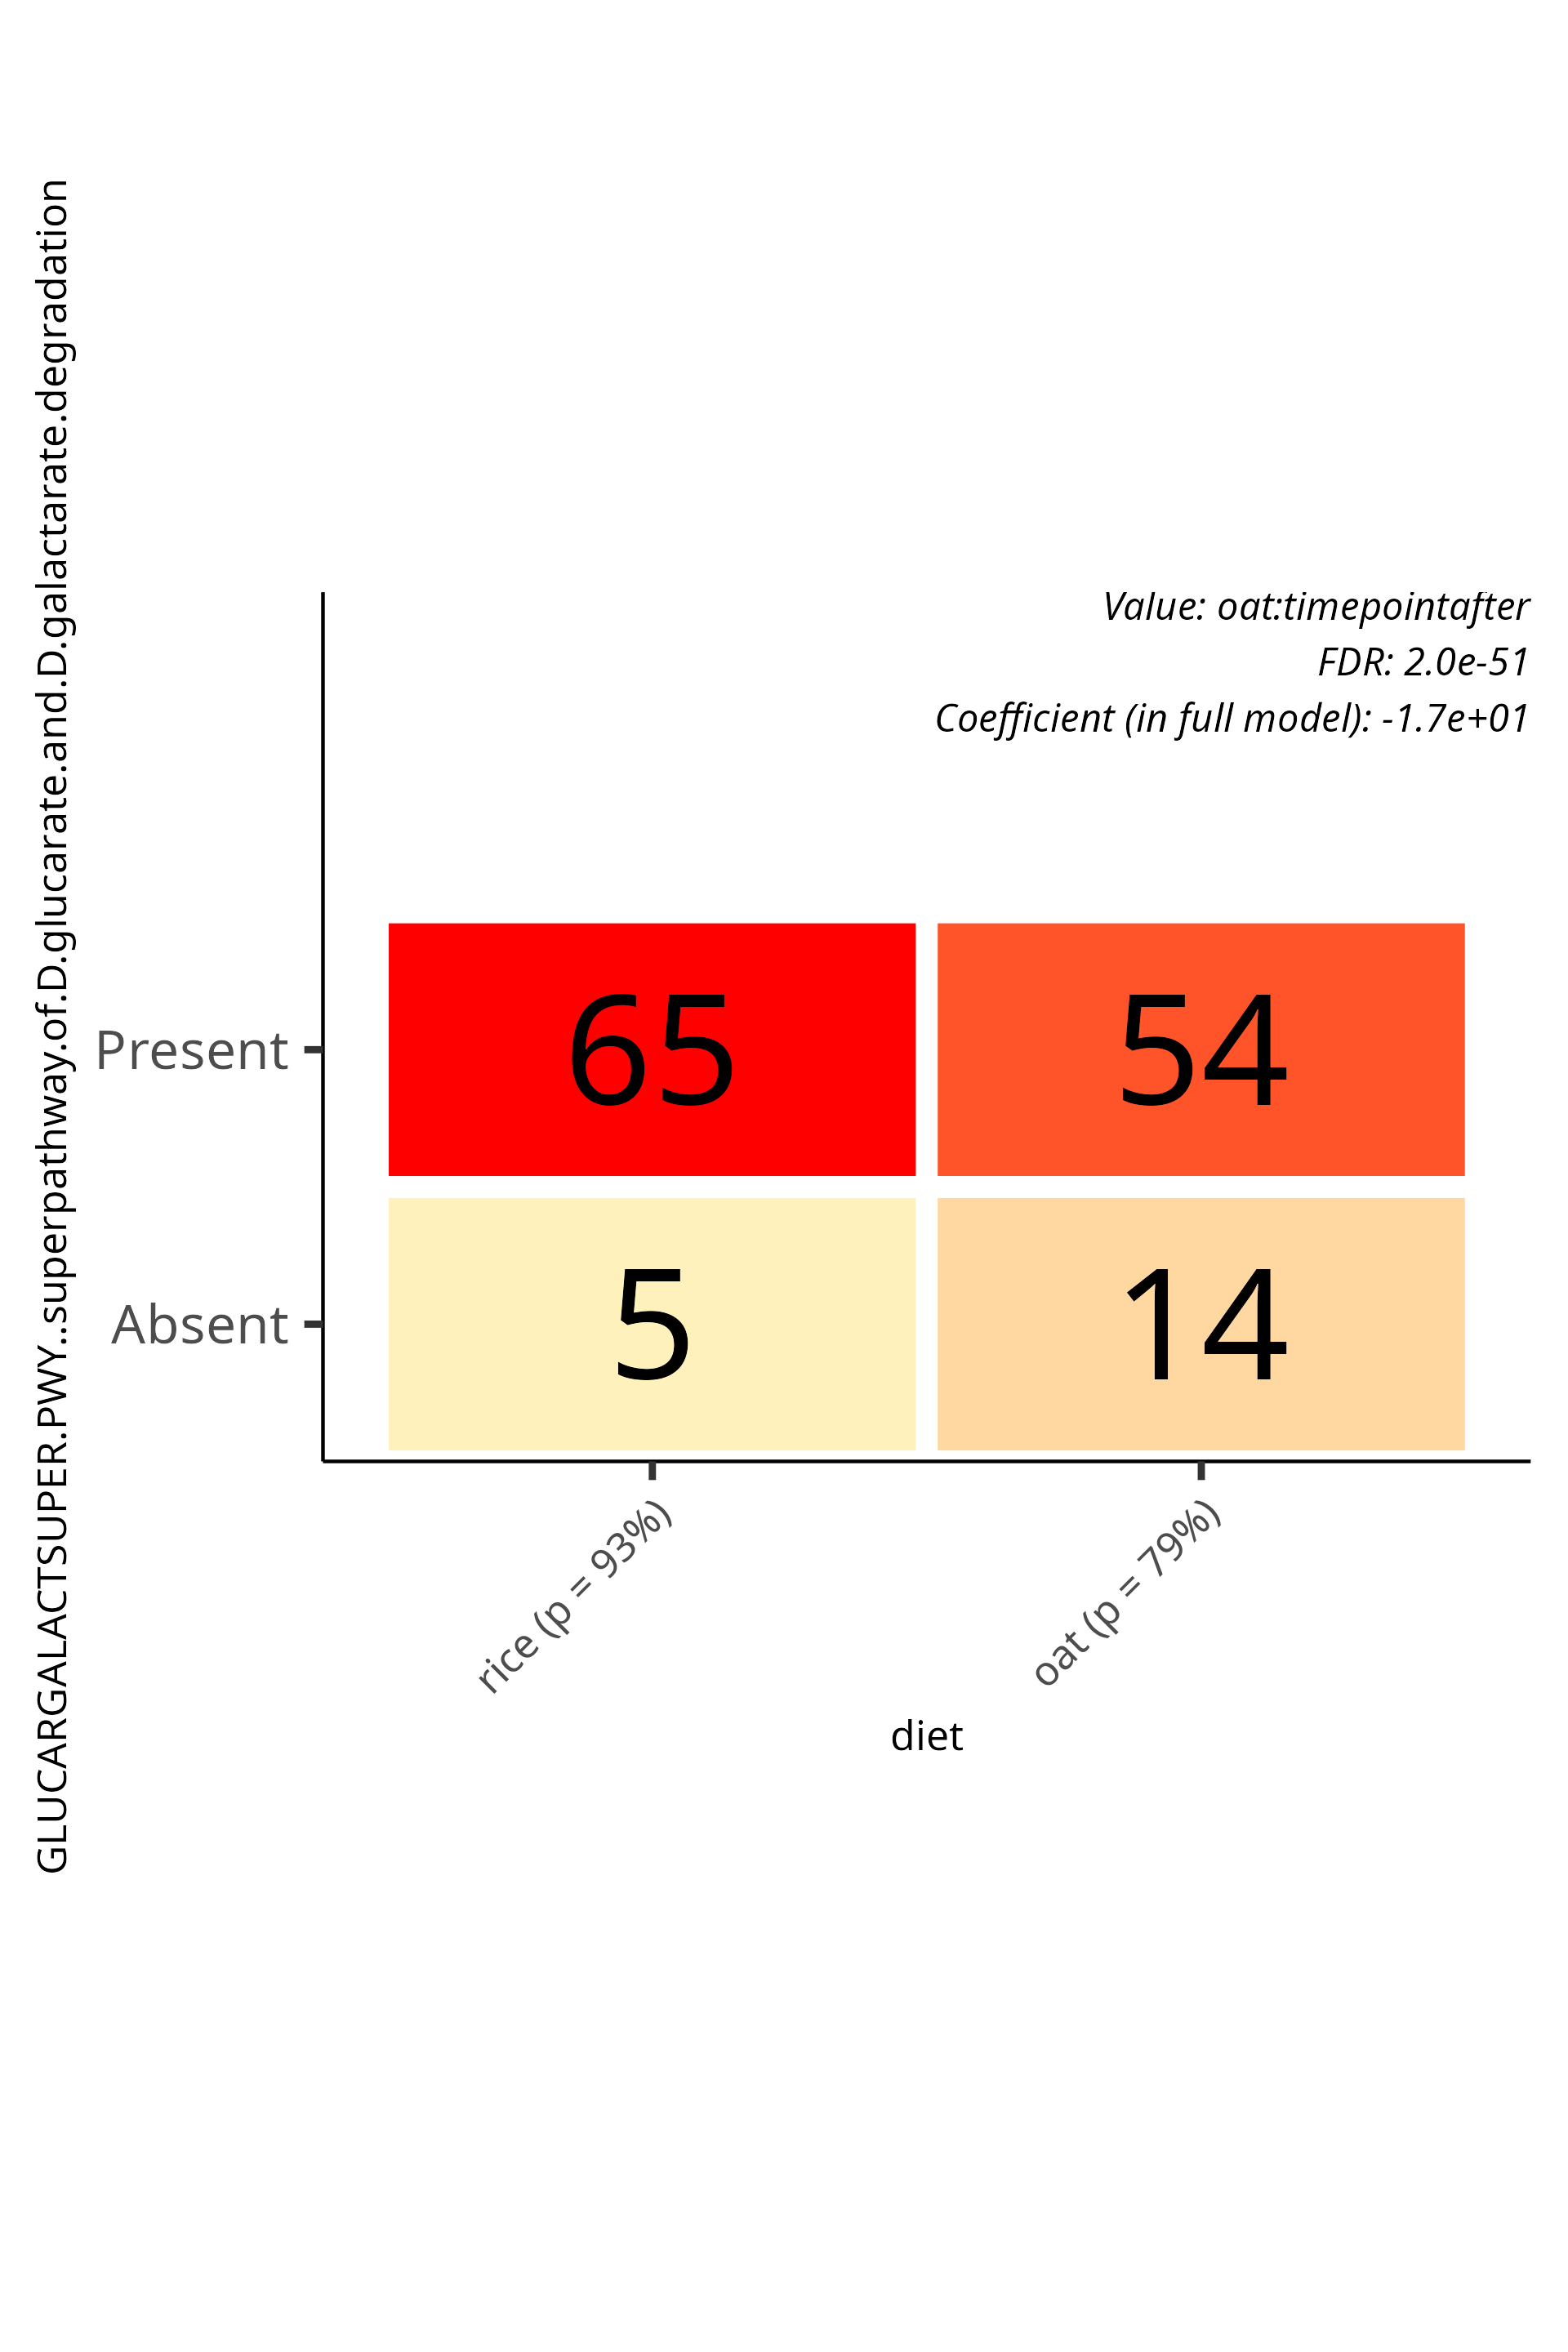
\includegraphics{../../output/daa/daa_pa/figures/association_plots/diet/logistic/diet_GLUCARGALACTSUPER.PWY..superpathway.of.D.glucarate.and.D.galactarate.degradation_logistic.png}
&
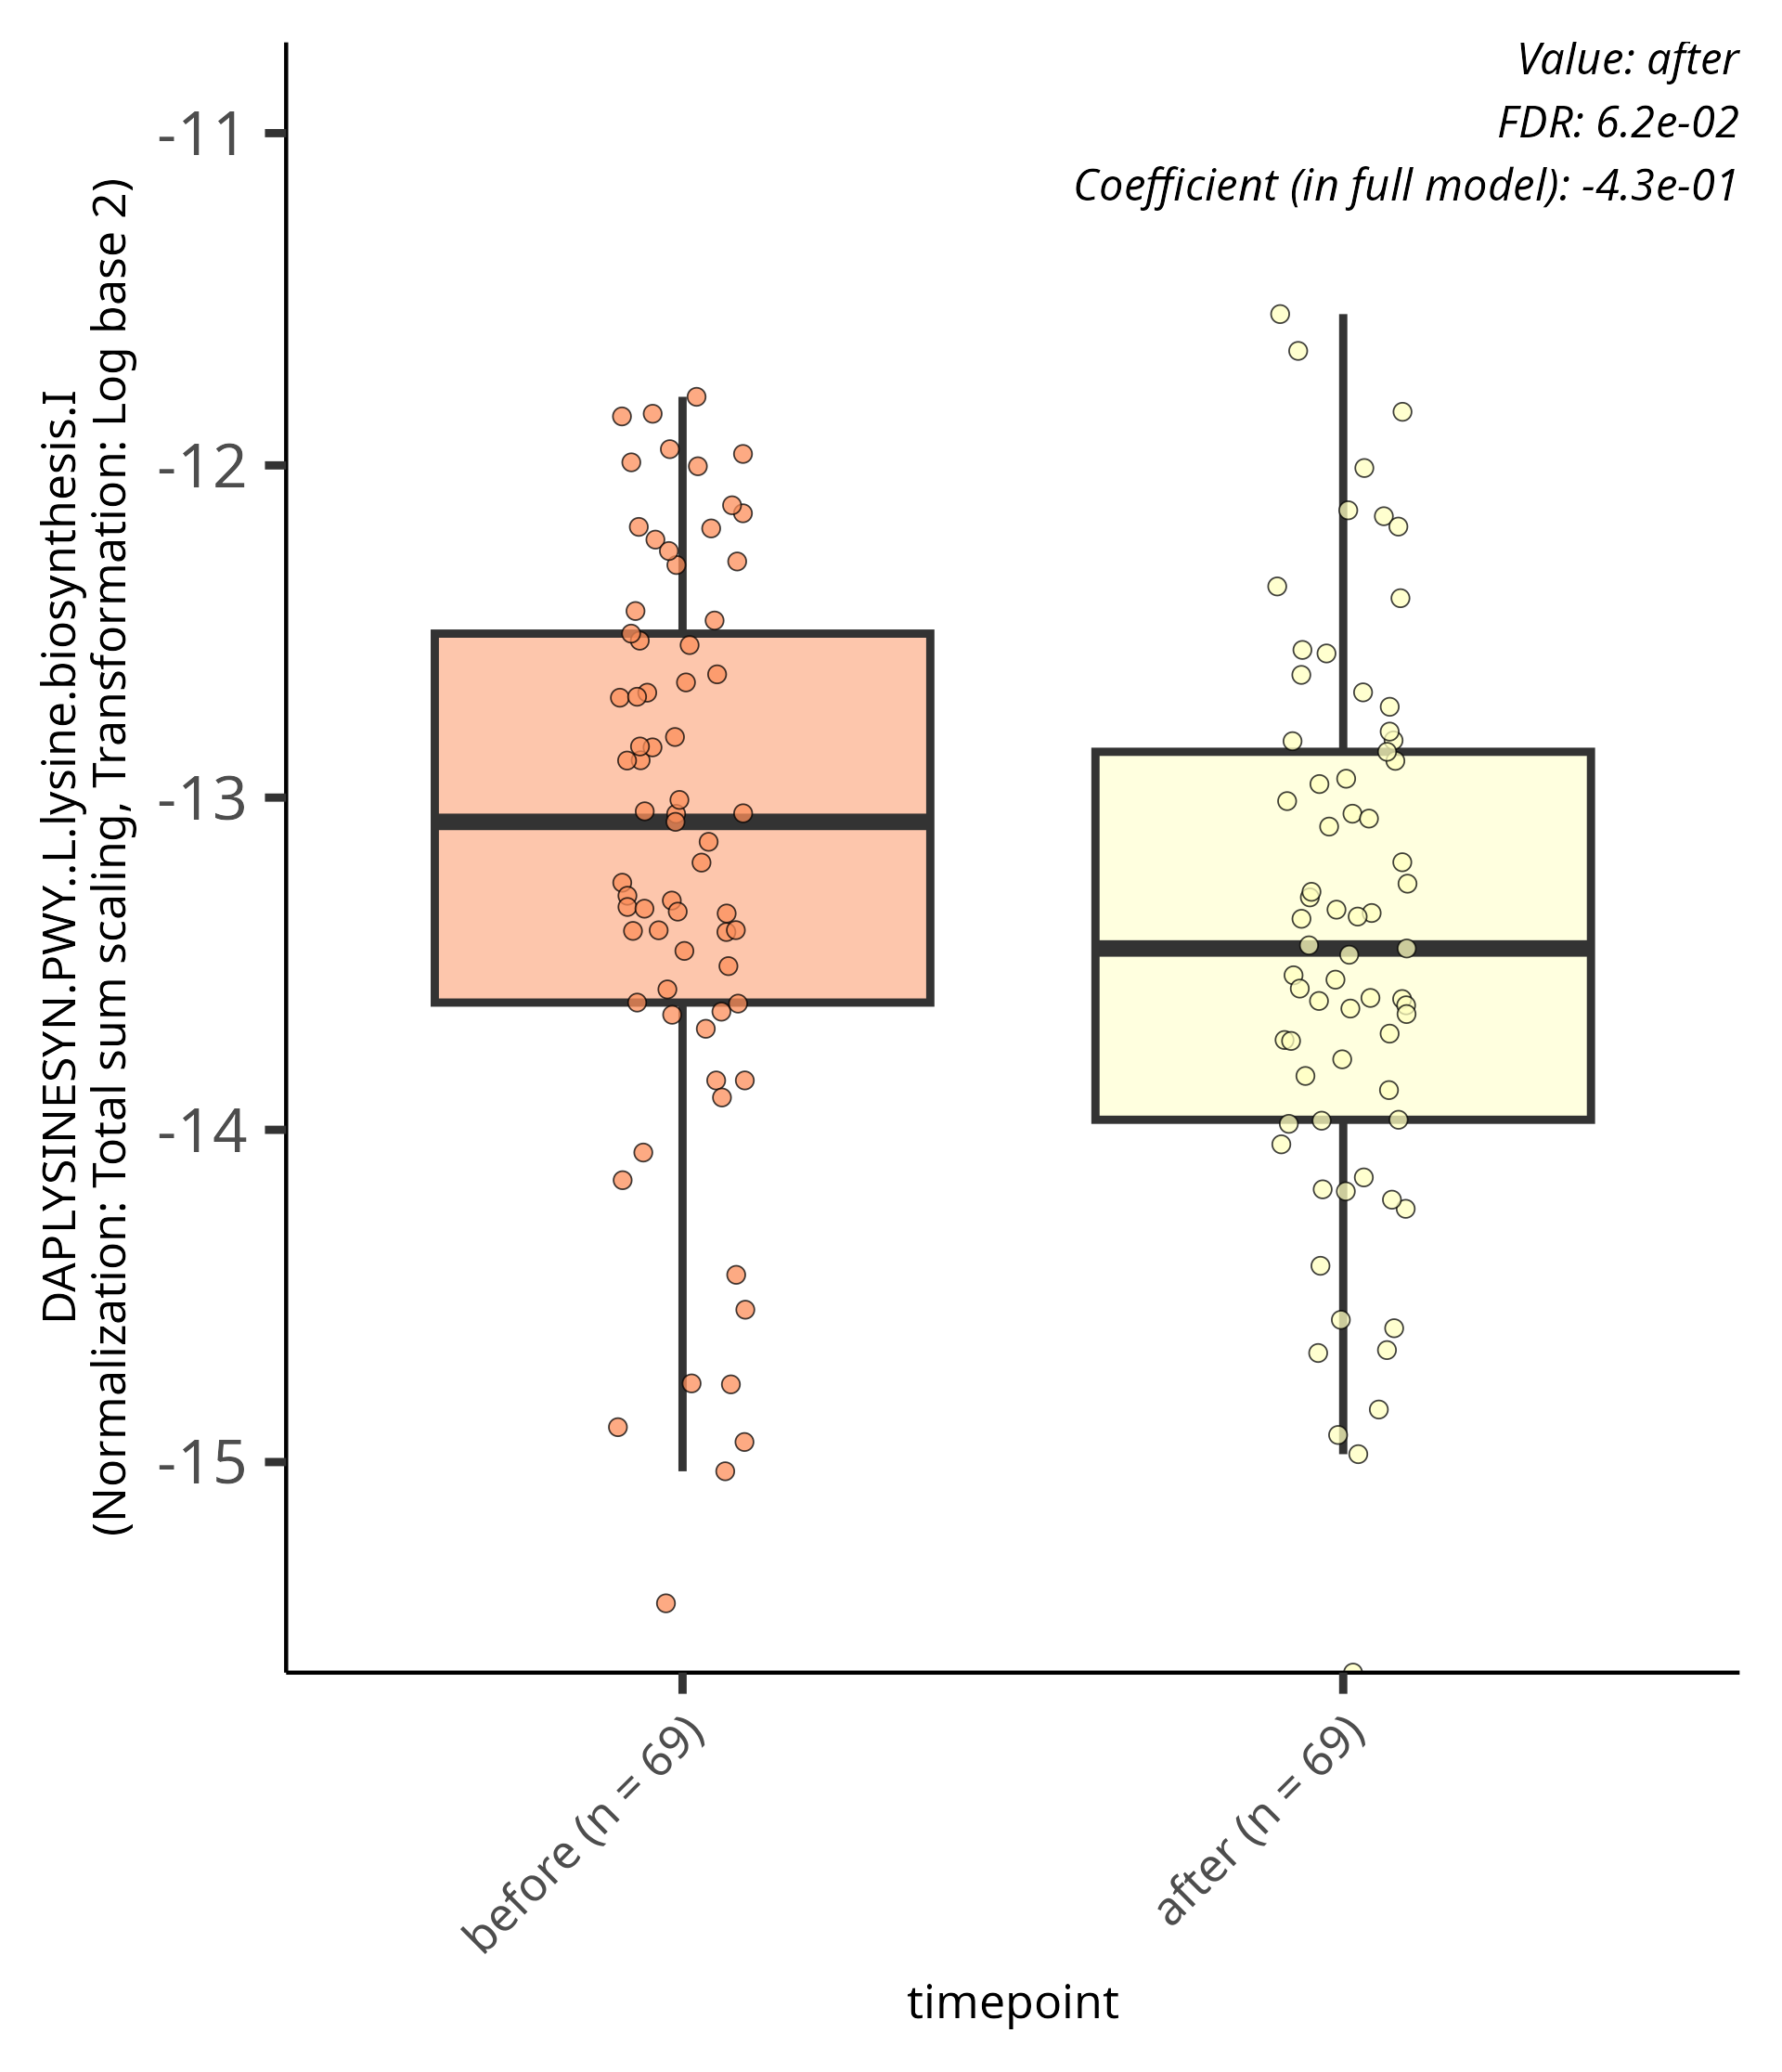
\includegraphics{../../output/daa/daa_pa/figures/association_plots/timepoint/linear/timepoint_DAPLYSINESYN.PWY..L.lysine.biosynthesis.I_linear.png} \\
\end{longtable}




\end{document}
